%# -*- coding: utf-8-unix -*-
%%==================================================
%% thesis.tex
%%==================================================

% 双面打印
\documentclass[bachelor, fontset=adobe, openright, oneside]{sjtuthesis}
% \documentclass[bachelor, fontset=adobe, openany, oneside, submit]{sjtuthesis}
% \documentclass[master, fontset=adobe, review]{sjtuthesis}
% \documentclass[%
%   bachelor|master|doctor,	% 必选项
%   fontset=adobe|windows,  	% 只测试了adobe
%   oneside|twoside,		% 单面打印,双面打印(奇偶页交换页边距,默认)
%   openany|openright, 		% 可以在奇数或者偶数页开新章|只在奇数页开新章(默认)
%   zihao=-4|5,, 		% 正文字号:小四、五号(默认)
%   review,	 		% 盲审论文,隐去作者姓名、学号、导师姓名、致谢、发表论文和参与的项目
%   submit			% 定稿提交的论文,插入签名扫描版的原创性声明、授权声明 
% ]

% 逐个导入参考文献数据库
\addbibresource{bib/thesis.bib}
% \addbibresource{bib/chap2.bib}

\begin{document}

%% 无编号内容:中英文论文封面、授权页
%# -*- coding: utf-8-unix -*-
\title{学术搜索引擎大规模查询系统的建立与优化}
\author{彭乾旸}
\advisor{甘小莺副教授}
% \coadvisor{某某教授}
\defenddate{2017年6月15日}
\school{上海交通大学}
\institute{计算机科学与工程系}
\studentnumber{5130309751}
\major{电子信息科学类}

\englishtitle{The Implementation and Optimization of Large-Scaled Academic Searching Platform}
\englishauthor{Qianyang Peng}
\englishadvisor{Xiaoying Gan}
% \englishcoadvisor{Prof. \textsc{Uom Uom}}
\englishschool{Shanghai Jiao Tong University}
\englishinstitute{\textsc{Depart of Computer Science and Engineering, School of Electronics, Information and Electrical Engineering} \\
  \textsc{Shanghai Jiao Tong University} \\
  \textsc{Shanghai, P.R.China}}
\englishmajor{IEEE Honor Class}
\englishdate{Jun. 15th, 2017}


\maketitle

\makeenglishtitle

\makeatletter
\ifsjtu@submit\relax
	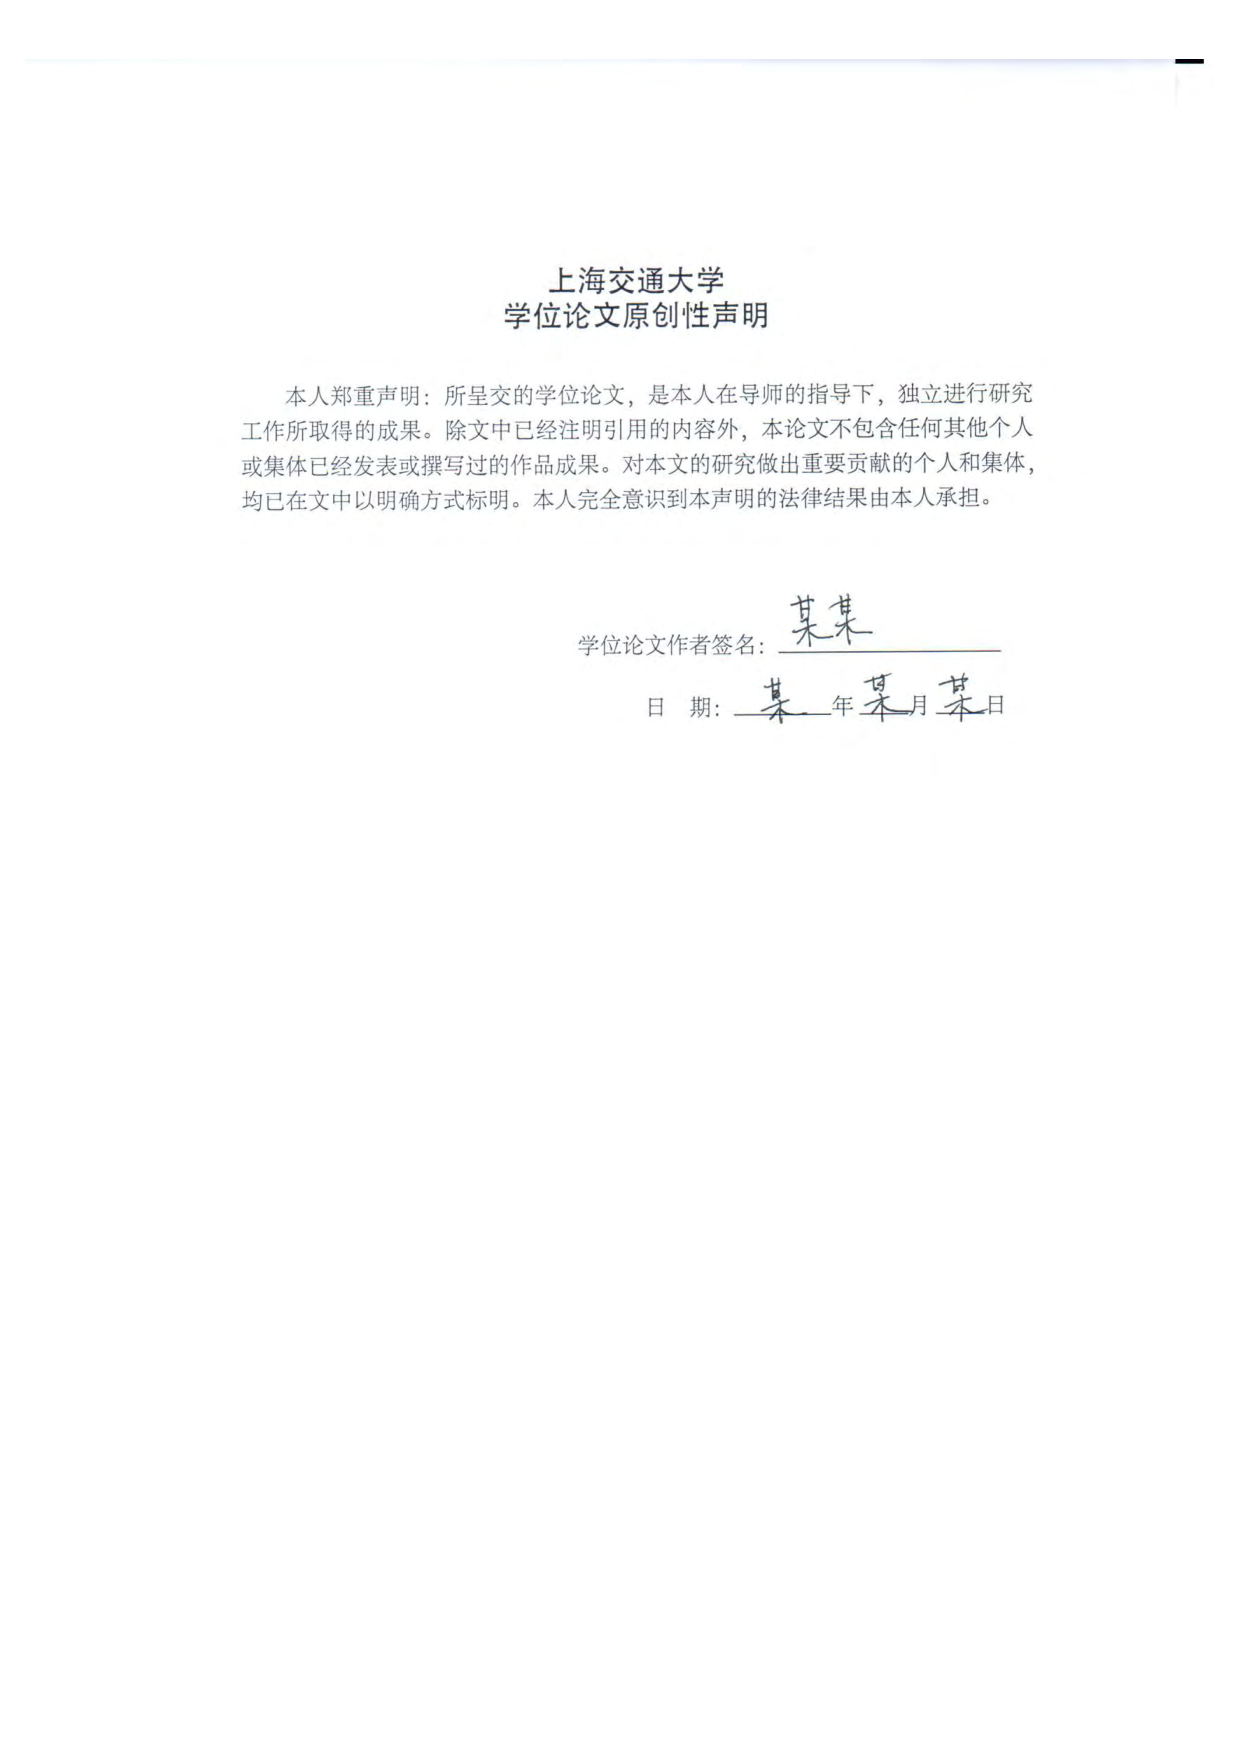
\includepdf{pdf/original.pdf}
	\cleardoublepage
	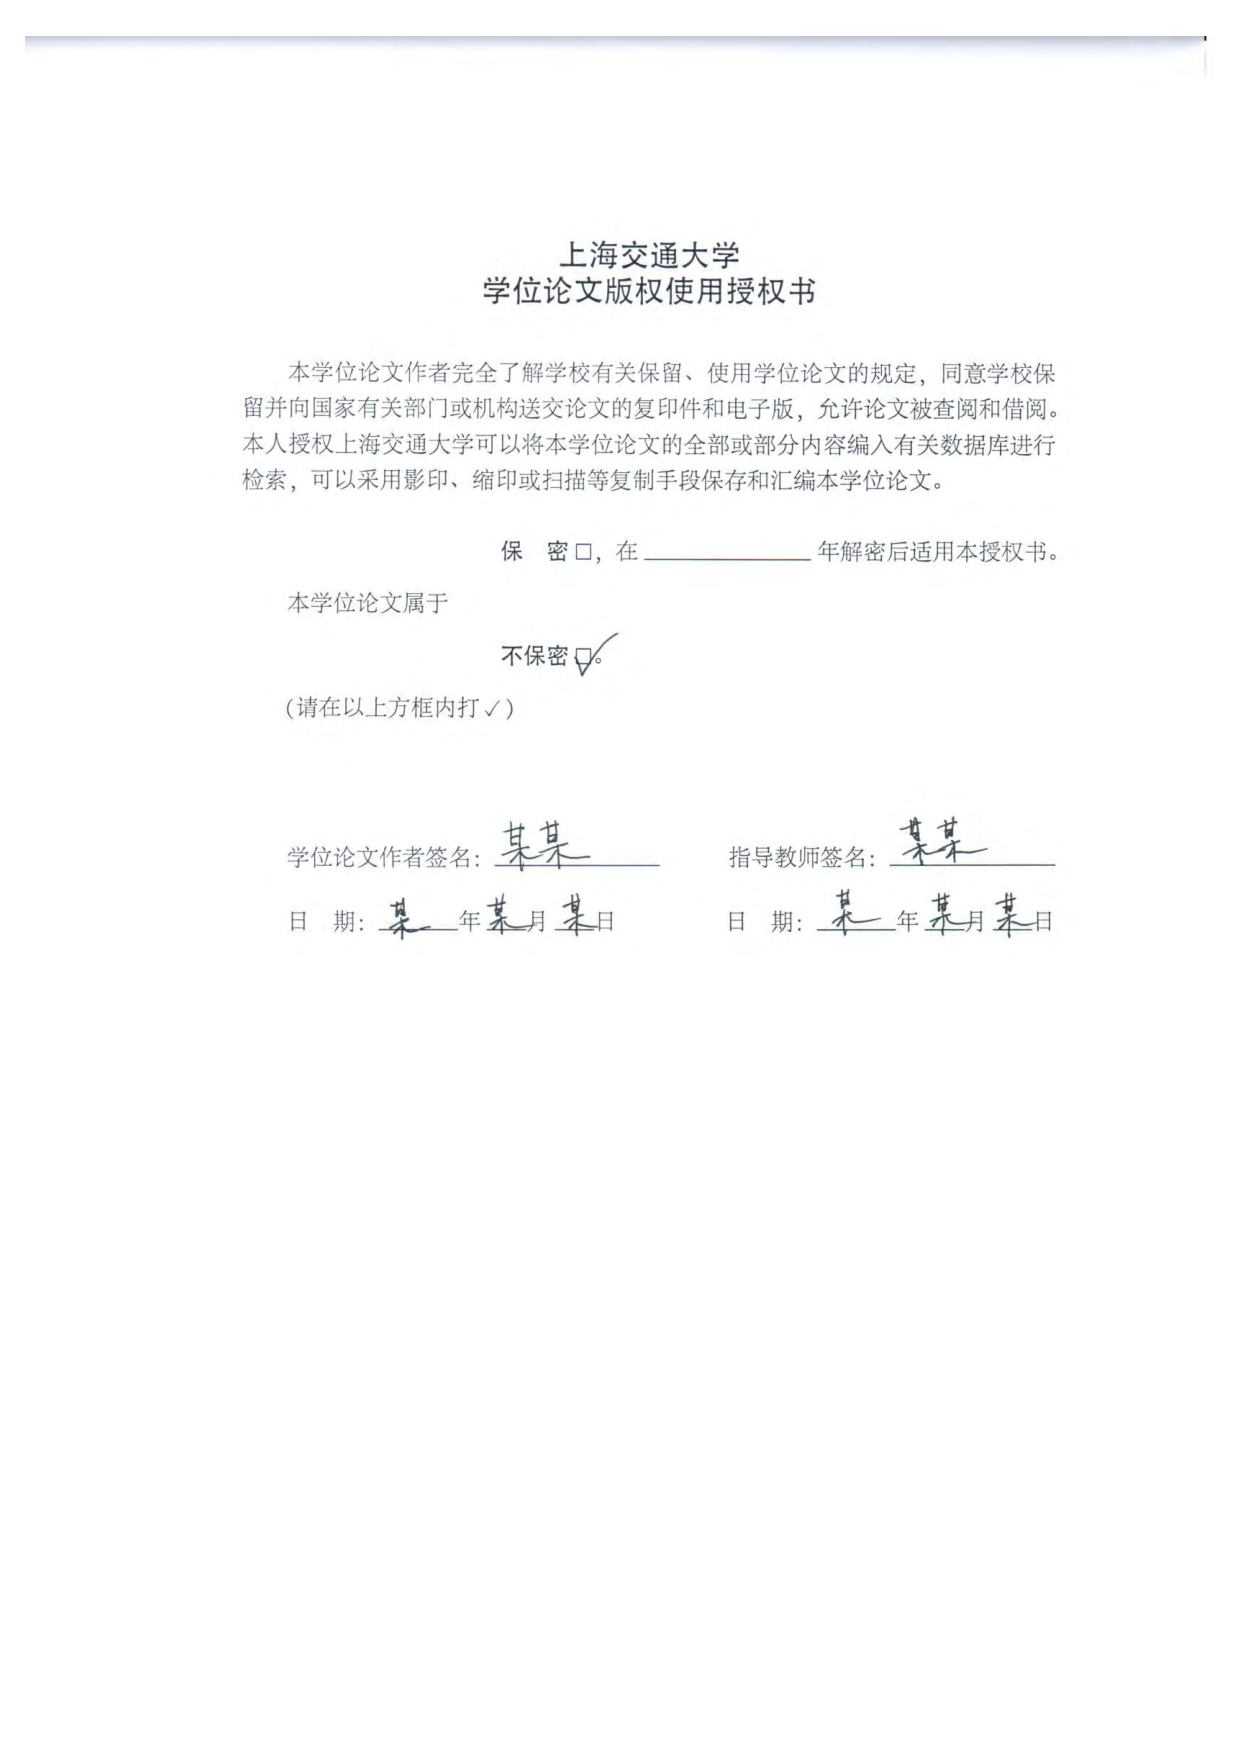
\includepdf{pdf/authorization.pdf}
	\cleardoublepage
\else
\ifsjtu@review\relax
% exclude the original claim and authorization
\else
	\makeDeclareOriginal
	\makeDeclareAuthorization
\fi
\fi
\makeatother


\frontmatter 	% 使用罗马数字对前言编号

%% 摘要
\pagestyle{main}
%# -*- coding: utf-8-unix -*-
%%==================================================
%% abstract.tex for SJTU Master Thesis
%%==================================================

\begin{abstract}

上海交通

\keywords{\large 上海交大 \quad 饮水思源 \quad 爱国荣校}
\end{abstract}

\begin{englishabstract}

An 

\englishkeywords{\large SJTU, master thesis, XeTeX/LaTeX template}
\end{englishabstract}



%% 目录、插图目录、表格目录
\tableofcontents
%\listoffigures
%\addcontentsline{toc}{chapter}{\listfigurename} %将插图目录加入全文目录
%\listoftables
%\addcontentsline{toc}{chapter}{\listtablename}  %将表格目录加入全文目录
%\listofalgorithms
%\addcontentsline{toc}{chapter}{算法索引}        %将算法目录加入全文目录

%%# -*- coding: utf-8-unix -*-
\chapter{主要符号对照表}
\label{chap:symb}

\begin{longtable}{rl}
$\epsilon$     & 介电常数 \\
 $\mu$ 		& 磁导率 \\
 $\epsilon$     & 介电常数 \\
 $\mu$ 		& 磁导率 \\
 $\epsilon$     & 介电常数 \\
 $\mu$ 		& 磁导率 \\
 $\epsilon$ 	& 介电常数 \\
 $\mu$ 		& 磁导率 \\
 $\epsilon$     & 介电常数 \\
 $\mu$ 		& 磁导率 \\
 $\epsilon$     & 介电常数 \\
 $\mu$ 		& 磁导率 \\
 $\epsilon$     & 介电常数 \\
 $\mu$ 		& 磁导率 \\
 $\epsilon$ 	& 介电常数 \\
 $\mu$ 		& 磁导率 \\
 $\epsilon$     & 介电常数 \\
 $\mu$ 		& 磁导率 \\
 $\epsilon$     & 介电常数 \\
 $\mu$ 		& 磁导率 \\
 $\epsilon$     & 介电常数 \\
 $\mu$ 		& 磁导率 \\
 $\epsilon$ 	& 介电常数 \\
 $\mu$ 		& 磁导率 \\
 $\epsilon$     & 介电常数 \\
 $\mu$ 		& 磁导率 \\
 $\epsilon$     & 介电常数 \\
 $\mu$ 		& 磁导率 \\
 $\epsilon$     & 介电常数 \\
 $\mu$ 		& 磁导率 \\
 $\epsilon$ 	& 介电常数 \\
 $\mu$ 		& 磁导率 \\
 $\epsilon$     & 介电常数 \\
 $\mu$ 		& 磁导率 \\
 $\epsilon$     & 介电常数 \\
 $\mu$ 		& 磁导率 \\
 $\epsilon$     & 介电常数 \\
 $\mu$ 		& 磁导率 \\
 $\epsilon$ 	& 介电常数 \\
 $\mu$ 		& 磁导率 \\
 $\epsilon$     & 介电常数 \\
 $\mu$ 		& 磁导率 \\
 $\epsilon$     & 介电常数 \\
 $\mu$ 		& 磁导率 \\
 $\epsilon$     & 介电常数 \\
 $\mu$ 		& 磁导率 \\
 $\epsilon$ 	& 介电常数 \\
 $\mu$ 		& 磁导率 \\
 $\epsilon$     & 介电常数 \\
 $\mu$ 		& 磁导率 \\
 $\epsilon$     & 介电常数 \\
 $\mu$ 		& 磁导率 \\
 $\epsilon$     & 介电常数 \\
 $\mu$ 		& 磁导率 \\
\end{longtable}
 % 主要符号、缩略词对照表

\mainmatter	% 使用阿拉伯数字对正文编号

%% 正文内容
\pagestyle{main}
%%# -*- coding: utf-8-unix -*-
%%==================================================
%% chapter01.tex for SJTU Master Thesis
%%==================================================

%\bibliographystyle{sjtu2}%[此处用于每章都生产参考文献]
\chapter{这是什么}
\label{chap:intro}

这是上海交通大学(非官方)学位论文 \LaTeX 模板,当前版本是 \version 。

最早的一版学位模板是一位热心的物理系同学制作的。
那份模板参考了自动化所学位论文模板,使用了CASthesis.cls文档类,中文字符处理则采用当时最为流行的 \CJKLaTeX 方案。
我根据交大研究生院对学位论文的要求
\footnote{\url{http://www.gs.sjtu.edu.cn/policy/fileShow.ahtml?id=130}}
,结合少量个人审美喜好,完成了一份基本可用的交大 \LaTeX 学位论文模板。
但是,搭建一个 \CJKLaTeX 环境并不简单,单单在Linux下配置环境和添加中文字体,就足够让新手打退堂鼓。
在William Wang的建议下,我开始着手把模板向 \XeTeX 引擎移植。
他完成了最初的移植,多亏了他出色的工作,后续的改善工作也得以顺利进行。

随着我对 \LaTeX 系统认知增加,我又断断续续做了一些完善模板的工作,在原有硕士学位论文模板的基础上完成了交大学士和博士学位论文模板。

现在,交大学位论文模板SJTUTHesis代码在github
\footnote{\url{https://github.com/weijianwen/SJTUThesis}}
上维护。
你可以\href{https://github.com/weijianwen/SJTUThesis/issues}{在github上开issue}
、或者在\href{https://bbs.sjtu.edu.cn/bbsdoc?board=TeX_LaTeX}{水源LaTeX版}发帖来反映遇到的问题。

\section{使用模板}

\subsection{准备工作}
\label{sec:requirements}

要使用这个模板撰写学位论文,需要在\emph{TeX系统}、\emph{中英文字体}、\emph{TeX技能}上有所准备。

\begin{itemize}[noitemsep,topsep=0pt,parsep=0pt,partopsep=0pt]
	\item {\TeX}系统:所使用的{\TeX}系统要支持 \XeTeX 引擎,且带有ctex 2.x宏包,以2015年的\emph{完整}TeXLive、MacTeX发行版为佳。
	\item 中英文字体:操作系统中需要安装\footnote{在Windows、Mac OS X 以及 Linux 上安装额外的字体,可以参考\href{https://www.searchfreefonts.com/articles/how-to-install-fonts.htm}{“How to install fonts?”}。
}TeX Gyre Termes字体\footnote{\url{http://www.gust.org.pl/projects/e-foundry/tex-gyre/termes}}和四款Adobe中文字体
\footnote{请从合法渠道获得Adobe字体。}:AdobeSongStd、AdobeKaitiStd、AdobeHeitiStd、AdobeFangsongStd。
	\item TeX技能:尽管提供了对模板的必要说明,但这不是一份“ \LaTeX 入门文档”。在使用前请先通读其他入门文档。
	\item 针对Windows用户的额外需求:学位论文模本分别使用git和GNUMake进行版本控制和构建,建议从Cygwin\footnote{\url{http://cygwin.com}}安装这两个工具。
\end{itemize}

\subsection{模板选项}
\label{sec:thesisoption}

sjtuthesis提供了一些常用选项,在thesis.tex在导入sjtuthesis模板类时,可以组合使用。
这些选项包括:

\begin{itemize}[noitemsep,topsep=0pt,parsep=0pt,partopsep=0pt]
\item 学位类型:bachelor(学位)、master(硕士)、doctor(博士),是必选项。
\item 中国字体:adobefonts(Adobe中文字体)、winfonts(使用Windows下的中文字体,该选项未在Linux/Mac下测试)。
\item 正文字号:cs4size(小四)、c5size(五号)。
\item 盲审选项:使用review选项后,论文作者、学号、导师姓名、致谢、发表论文和参与项目将被隐去。
\end{itemize}

\subsection{编译模板}
\label{sec:process}

模板默认使用GNUMake构建,GNUMake将调用latemk工具自动完成模板多轮编译:

\begin{lstlisting}[basicstyle=\small\ttfamily, caption={编译模板}, numbers=none]
make clean thesis.pdf
\end{lstlisting}

若需要生成包含“原创性声明扫描件”的学位论文文档,请将扫描件保存为statement.pdf,然后调用make生成submit.pdf。

\begin{lstlisting}[basicstyle=\small\ttfamily, caption={生成用于提交的学位论文}, numbers=none]
make clean submit.pdf
\end{lstlisting}

编译失败时,可以尝试手动逐次编译,定位故障。

\begin{lstlisting}[basicstyle=\small\ttfamily, caption={手动逐次编译}, numbers=none]
xelatex -no-pdf thesis
biber --debug thesis
xelatex thesis
xelatex thesis
\end{lstlisting}

\subsection{模板文件布局}
\label{sec:layout}

\begin{lstlisting}[basicstyle=\small\ttfamily,caption={模板文件布局},label=layout,float,numbers=none]
├── LICENSE
├── Makefile
├── README.md
├── bib
│   ├── chap1.bib
│   └── chap2.bib
├── bst
│   └── GBT7714-2005NLang.bst
├── figure
│   ├── chap2
│   │   ├── sjtulogo.eps
│   │   ├── sjtulogo.jpg
│   │   ├── sjtulogo.pdf
│   │   └── sjtulogo.png
│   └── sjtubanner.png
├── sjtuthesis.cfg
├── sjtuthesis.cls
├── statement.pdf
├── submit.pdf
├── tex
│   ├── abstract.tex
│   ├── ack.tex
│   ├── app_cjk.tex
│   ├── app_eq.tex
│   ├── app_log.tex
│   ├── chapter01.tex
│   ├── chapter02.tex
│   ├── chapter03.tex
│   ├── conclusion.tex
│   ├── id.tex
│   ├── patents.tex
│   ├── projects.tex
│   ├── pub.tex
│   └── symbol.tex
└── thesis.tex
\end{lstlisting}

本节介绍学位论文模板中木要文件和目录的功能。

\subsubsection{格式控制文件}
\label{sec:format}

格式控制文件控制着论文的表现形式,包括以下几个文件:
sjtuthesis.cfg, sjtuthesis.cls和GBT7714-2005NLang.bst。
其中,“cfg”和“cls”控制论文主体格式,“bst”控制参考文献条目的格式,

\subsubsection{主控文件thesis.tex}
\label{sec:thesistex}

主控文件thesis.tex的作用就是将你分散在多个文件中的内容“整合”成一篇完整的论文。
使用这个模板撰写学位论文时,你的学位论文内容和素材会被“拆散”到各个文件中:
譬如各章正文、各个附录、各章参考文献等等。
在thesis.tex中通过“include”命令将论文的各个部分包含进来,从而形成一篇结构完成的论文。
对模板定制时引入的宏包,建议放在导言区。

\subsubsection{各章源文件tex}
\label{sec:thesisbody}

这一部分是论文的主体,是以“章”为单位划分的,包括:

\begin{itemize}[noitemsep,topsep=0pt,parsep=0pt,partopsep=0pt]
	\item 中英文摘要(abstract.tex)。前言(frontmatter)的其他部分,中英文封面、原创性声明、授权信息在sjtuthesis.cls中定义,不单独分离为tex文件。
不单独弄成文件。
	\item 正文(mainmatter)——学位论文正文的各章内容,源文件是chapter\emph{xxx}.tex。
	\item 附录(app\emph{xx}.tex)、致谢(thuanks.tex)、攻读学位论文期间发表的学术论文目录(pub.tex)、个人简历(resume.tex)组成正文后的部分(backmatter)。
参考文献列表由bibtex插入,不作为一个单独的文件。
\end{itemize}

\subsubsection{图片文件夹figure}
\label{sec:fig}

figure文件夹放置了需要插入文档中的图片文件(支持PNG/JPG/PDF/EPS格式的图片),可以在按照章节划分子目录。
模板文件中使用\verb|\graphicspath|命令定义了图片存储的顶层目录,在插入图片时,顶层目录名“figure”可省略。

\subsubsection{参考文献数据库bib}
\label{sec:bib}

目前参考文件数据库目录只存放一个参考文件数据库thesis.bib。
关于参考文献引用,可参考第\ref{chap:example}章中的例子。


%%# -*- coding: utf-8-unix -*-
%%==================================================
%% chapter02.tex for SJTU Master Thesis
%% based on CASthesis
%% modified by wei.jianwen@gmail.com
%% Encoding: UTF-8
%%==================================================

\chapter{ \LaTeX 排版例子}
\label{chap:example}

\section{列表环境}
\label{sec:list}

\subsection{无序列表}
\label{sec:unorderlist}

以下是一个无序列表的例子,列表的每个条目单独分段。

\begin{itemize}
  \item 这是一个无序列表。
  \item 这是一个无序列表。
  \item 这是一个无序列表。
\end{itemize}

使用\verb+itemize*+环境可以创建行内无序列表。
\begin{itemize*}
  \item 这是一个无序列表。
  \item 这是一个无序列表。
  \item 这是一个无序列表。
\end{itemize*}
行内无序列表条目不单独分段,所有内容直接插入在原文的段落中。

\subsection{有序列表}
\label{sec:orderlist}

使用环境\verb+enumerate+和\verb+enumerate*+创建有序列表,
使用方法无序列表类似。

\begin{enumerate}
  \item 这是一个有序列表。
  \item 这是一个有序列表。
  \item 这是一个有序列表。
\end{enumerate}

使用\verb+enumerate*+环境可以创建行内有序列表。
\begin{enumerate*}
  \item 这是一个默认有序列表。
  \item 这是一个默认有序列表。
  \item 这是一个默认有序列表。
\end{enumerate*}
行内有序列表条目不单独分段,所有内容直接插入在原文的段落中。

\subsection{描述型列表}

使用环境\verb+description+可创建带有主题词的列表,条目语法是\verb+\item[主题] 内容+。
\begin{description}
    \item[主题一] 详细内容
    \item[主题二] 详细内容
    \item[主题三] 详细内容 \ldots
\end{description}

\subsection{自定义列表样式}

可以使用\verb+label+参数控制列表的样式,
详细可以参考WikiBooks\footnote{\url{https://en.wikibooks.org/wiki/LaTeX/List_Structures\#Customizing_lists}}。
比如一个自定义样式的行内有序列表
\begin{enumerate*}[label=\itshape\alph*)\upshape]
  \item 这是一个自定义样式有序列表。
  \item 这是一个自定义样式有序列表。
  \item 这是一个自定义样式有序列表。
\end{enumerate*}

\section{数学排版}
\label{sec:matheq}

\subsection{公式排版}
\label{sec:eqformat}

这里有举一个长公式排版的例子,来自\href{http://www.tex.ac.uk/tex-archive/info/math/voss/mathmode/Mathmode.pdf}{《Math mode》}:

\begin {multline}
  \frac {1}{2}\Delta (f_{ij}f^{ij})=
  2\left (\sum _{i<j}\chi _{ij}(\sigma _{i}-
    \sigma _{j}) ^{2}+ f^{ij}\nabla _{j}\nabla _{i}(\Delta f)+\right .\\
  \left .+\nabla _{k}f_{ij}\nabla ^{k}f^{ij}+
    f^{ij}f^{k}\left [2\nabla _{i}R_{jk}-
      \nabla _{k}R_{ij}\right ]\vphantom {\sum _{i<j}}\right )
\end{multline}

\subsection{SI单位}

使用\verb+siunitx+宏包可以方便地输入SI单位制单位,例如\verb+\SI{5}{\um}+可以得到\SI{5}{\um}。

\subsubsection{一个四级标题}
\label{sec:depth4}

这是全文唯一的一个四级标题。在这部分中将演示了mathtools宏包中可伸长符号(箭头、等号的例子)的例子。

\begin{displaymath}
    A \xleftarrow[n=0]{} B \xrightarrow[LongLongLongLong]{n>0} C 
\end{displaymath}

\begin{eqnarray}
  f(x) & \xleftrightarrow[]{A=B}  & B \\
  & \xleftharpoondown[below]{above} & B \nonumber \\
  & \xLeftrightarrow[below]{above} & B
\end{eqnarray}

又如:

\begin{align}
  \label{eq:none}
  & I(X_3;X_4)-I(X_3;X_4\mid{}X_1)-I(X_3;X_4\mid{}X_2) \nonumber \\
  = & [I(X_3;X_4)-I(X_3;X_4\mid{}X_1)]-I(X_3;X_4\mid{}\tilde{X}_2) \\
  = & I(X_1;X_3;X_4)-I(X_3;X_4\mid{}\tilde{X}_2)
\end{align}

\subsection{定理环境}

模板中定义了丰富的定理环境
algo(算法),thm(定理),lem(引理),prop(命题),cor(推论),defn(定义),conj(猜想),exmp(例),rem(注),case(情形),
bthm(断言定理),blem(断言引理),bprop(断言命题),bcor(断言推论)。
amsmath还提供了一个proof(证明)的环境。
这里举一个“定理”和“证明”的例子。
\begin{thm}[留数定理]
\label{thm:res}
  假设$U$是复平面上的一个单连通开子集,$a_1,\ldots,a_n$是复平面上有限个点,$f$是定义在$U\backslash \{a_1,\ldots,a_n\}$上的全纯函数,
  如果$\gamma$是一条把$a_1,\ldots,a_n$包围起来的可求长曲线,但不经过任何一个$a_k$,并且其起点与终点重合,那么:

  \begin{equation}
    \label{eq:res}
    \ointop_{\gamma}f(z)\,\mathrm{d}z = 2\uppi\mathbf{i}\sum^n_{k=1}\mathrm{I}(\gamma,a_k)\mathrm{Res}(f,a_k)
  \end{equation}

  如果$\gamma$是若尔当曲线,那么$\mathrm{I}(\gamma, a_k)=1$,因此:

  \begin{equation}
    \label{eq:resthm}
    \ointop_{\gamma}f(z)\,\mathrm{d}z = 2\uppi\mathbf{i}\sum^n_{k=1}\mathrm{Res}(f,a_k)
  \end{equation}

      % \oint_\gamma f(z)\, dz = 2\pi i \sum_{k=1}^n \mathrm{Res}(f, a_k ). 

  在这里,$\mathrm{Res}(f, a_k)$表示$f$在点$a_k$的留数,$\mathrm{I}(\gamma,a_k)$表示$\gamma$关于点$a_k$的卷绕数。
  卷绕数是一个整数,它描述了曲线$\gamma$绕过点$a_k$的次数。如果$\gamma$依逆时针方向绕着$a_k$移动,卷绕数就是一个正数,
  如果$\gamma$根本不绕过$a_k$,卷绕数就是零。

  定理\ref{thm:res}的证明。
  
  \begin{proof}
    首先,由……

    其次,……

    所以……
  \end{proof}
\end{thm}

上面的公式例子中,有一些细节希望大家注意。微分号d应该使用“直立体”也就是用mathrm包围起来。
并且,微分号和被积函数之间应该有一段小间隔,可以插入\verb+\,+得到。
斜体的$d$通常只作为一般变量。
i,j作为虚数单位时,也应该使用“直立体”为了明显,还加上了粗体,例如\verb+\mathbf{i}+。斜体$i,j$通常用作表示“序号”。
其他字母在表示常量时,也推荐使用“直立体”譬如,圆周率$\uppi$(需要upgreek宏包),自然对数的底$\mathrm{e}$。
不过,我个人觉得斜体的$e$和$\pi$很潇洒,在不至于引起混淆的情况下,我也用这两个字母的斜体表示对应的常量。


\section{向文档中插入图像}
\label{sec:insertimage}

\subsection{支持的图片格式}
\label{sec:imageformat}

\XeTeX 可以很方便地插入PDF、PNG、JPG格式的图片。

插入PNG/JPG的例子如\ref{fig:SRR}所示。
这两个水平并列放置的图共享一个“图标题”(table caption),没有各自的小标题。

\begin{figure}[!htp]
  \centering
  
\includegraphics[width=0.3\textwidth]{example/sjtulogo.png}
  \hspace{1cm}
  
\includegraphics[width=0.3\textwidth]{example/sjtulogo.jpg}
  \bicaption[fig:SRR]{这里将出现在插图索引中}{中文题图}{Fig}{English caption}
\end{figure}

% 这里还有插入eps图像和pdf图像的例子,如图\ref{fig:epspdf:a}和图\ref{fig:epspdf:b}。这里将EPS和PDF图片作为子图插入,每个子图有自己的小标题。并列子图的功能是使用subfigure宏包提供的。
% 
% \begin{figure}
%   \centering
%   \subfigure[EPS Figure]{
%     \label{fig:epspdf:a} %% label for first subfigure
%     
\includegraphics[width=0.3\textwidth]{example/sjtulogo.eps}}
%   \hspace{1in}
%   \subfigure[PDF Figure]{
%     \label{fig:epspdf:b} %% label for second subfigure
%     
\includegraphics[width=0.3\textwidth]{example/sjtulogo.pdf}}
%   \bicaption[fig:pdfeps]{插入eps图像和pdf图像}{插入eps和pdf的例子}{Fig}{An EPS and PDF demo}
% \end{figure}

更多关于 \LaTeX 插图的例子可以参考\href{http://www.cs.duke.edu/junhu/Graphics3.pdf}{《\LaTeX 插图指南》}。

\subsection{长标题的换行}
\label{sec:longcaption}

图\ref{fig:longcaptionbad}和图\ref{fig:longcaptiongood}都有比较长图标题,通过对比发现,图\ref{fig:longcaptiongood}的换行效果更好一些。
其中使用了minipage环境来限制整个浮动体的宽度。

\begin{figure}[!htp]
 \centering
 
\includegraphics[width=4cm]{example/sjtulogo.pdf}
 \bicaption[fig:longcaptionbad]{这里将出现在插图索引}{海交通大学是我国历史最悠久的高等学府之一,是教育部直属、教育部与上海市共建的全国重点大学.}{Fig}{Where there is a will, there is a way.}
\end{figure}

\begin{figure}[!htbp]
  \centering
  \begin{minipage}[b]{0.6\textwidth}
    \captionstyle{\centering}
    \centering
    
\includegraphics[width=4cm]{example/sjtulogo.pdf}
    \bicaption[fig:longcaptiongood]{这里将出现在插图索引}{海交通大学是我国历史最悠久的高等学府之一,是教育部直属、教育部与上海市共建的全国重点大学.}{Fig}{Where there is a will, there is a way.}
  \end{minipage}     
\end{figure}

\subsection{绘制流程图}

图\ref{fig:flow_chart}是一张流程图示意。使用tikz环境,搭配四种预定义节点(\verb+startstop+、\verb+process+、\verb+decision+和\verb+io+),可以容易地绘制出流程图。
\begin{figure}[!htp]
    \centering
    \resizebox{6cm}{!}{\begin{tikzpicture}[node distance=2cm]
    \node (pic) [startstop] {待测图片};
    \node (bg) [io, below of=pic] {读取背景};
    \node (pair) [process, below of=bg] {匹配特征点对};
    \node (threshold) [decision, below of=pair, yshift=-0.5cm] {多于阈值};
    \node (clear) [decision, right of=threshold, xshift=3cm] {清晰?};
    \node (capture) [process, right of=pair, xshift=3cm, yshift=0.5cm] {重采};
    \node (matrix_p) [process, below of=threshold, yshift=-0.8cm] {透视变换矩阵};
    \node (matrix_a) [process, right of=matrix_p, xshift=3cm] {仿射变换矩阵};
    \node (reg) [process, below of=matrix_p] {图像修正};
    \node (return) [startstop, below of=reg] {配准结果};
     
    %连接具体形状
    \draw [arrow](pic) -- (bg);
    \draw [arrow](bg) -- (pair);
    \draw [arrow](pair) -- (threshold);

    \draw [arrow](threshold) -- node[anchor=south] {否} (clear);

    \draw [arrow](clear) -- node[anchor=west] {否} (capture);
    \draw [arrow](capture) |- (pic);
    \draw [arrow](clear) -- node[anchor=west] {是} (matrix_a);
    \draw [arrow](matrix_a) |- (reg);

    \draw [arrow](threshold) -- node[anchor=east] {是} (matrix_p);
    \draw [arrow](matrix_p) -- (reg);
    \draw [arrow](reg) -- (return);
\end{tikzpicture}
}
    \bicaption[fig:flow_chart]{绘制流程图效果}{流程图}{Fig}{Flow chart}
\end{figure}
  
\clearpage

\section{表格}
\label{sec:tab}

这一节给出的是一些表格的例子,如表\ref{tab:firstone}所示。

\begin{table}[!hpb]
  \centering
  \bicaption[tab:firstone]{指向一个表格的表目录索引}{一个颇为标准的三线表格\footnotemark[1]}{Table}{A Table}
  \begin{tabular}{@{}llr@{}} \toprule
    \multicolumn{2}{c}{Item} \\ \cmidrule(r){1-2}
    Animal & Description & Price (\$)\\ \midrule
    Gnat & per gram & 13.65 \\
    & each & 0.01 \\
    Gnu & stuffed & 92.50 \\
    Emu & stuffed & 33.33 \\
    Armadillo & frozen & 8.99 \\ \bottomrule
  \end{tabular}
\end{table}
\footnotetext[1]{这个例子来自\href{http://www.ctan.org/tex-archive/macros/latex/contrib/booktabs/booktabs.pdf}{《Publication quality tables in LATEX》}(booktabs宏包的文档)。这也是一个在表格中使用脚注的例子,请留意与threeparttable实现的效果有何不同。}

下面一个是一个更复杂的表格,用threeparttable实现带有脚注的表格,如表\ref{tab:footnote}。

\begin{table}[!htpb]
  \bicaption[tab:footnote]{出现在表目录的标题}{一个带有脚注的表格的例子}{Table}{A Table with footnotes}
  \centering
  \begin{threeparttable}[b]
     \begin{tabular}{ccd{4}cccc}
      \toprule
      \multirow{2}{6mm}{total}&\multicolumn{2}{c}{20\tnote{1}} & \multicolumn{2}{c}{40} &  \multicolumn{2}{c}{60}\\
      \cmidrule(lr){2-3}\cmidrule(lr){4-5}\cmidrule(lr){6-7}
      &www & k & www & k & www & k \\
      \midrule
      &$\underset{(2.12)}{4.22}$ & 120.0140\tnote{2} & 333.15 & 0.0411 & 444.99 & 0.1387 \\
      &168.6123 & 10.86 & 255.37 & 0.0353 & 376.14 & 0.1058 \\
      &6.761    & 0.007 & 235.37 & 0.0267 & 348.66 & 0.1010 \\
      \bottomrule
    \end{tabular}
    \begin{tablenotes}
    \item [1] the first note.% or \item [a]
    \item [2] the second note.% or \item [b]
    \end{tablenotes}
  \end{threeparttable}
\end{table}

\section{参考文献管理}

 \LaTeX 具有将参考文献内容和表现形式分开管理的能力,涉及三个要素:参考文献数据库、参考文献引用格式、在正文中引用参考文献。
这样的流程需要多次编译:

\begin{enumerate}[noitemsep,topsep=0pt,parsep=0pt,partopsep=0pt]
	\item 用户将论文中需要引用的参考文献条目,录入纯文本数据库文件(bib文件)。
	\item 调用xelatex对论文模板做第一次编译,扫描文中引用的参考文献,生成参考文献入口文件(aux)文件。
	\item 调用bibtex,以参考文献格式和入口文件为输入,生成格式化以后的参考文献条目文件(bib)。
	\item 再次调用xelatex编译模板,将格式化以后的参考文献条目插入正文。
\end{enumerate}

参考文献数据库(thesis.bib)的条目,可以从Google Scholar搜索引擎\footnote{\url{https://scholar.google.com}}、CiteSeerX搜索引擎\footnote{\url{http://citeseerx.ist.psu.edu}}中查找,文献管理软件Papers\footnote{\url{http://papersapp.com}}、Mendeley\footnote{\url{http://www.mendeley.com}}、JabRef\footnote{\url{http://jabref.sourceforge.net}}也能够输出条目信息。

下面是在Google Scholar上搜索到的一条文献信息,格式是纯文本:

\begin{lstlisting}[caption={从Google Scholar找到的参考文献条目}, label=googlescholar, escapeinside="", numbers=none]
    @phdthesis{"白2008信用风险传染模型和信用衍生品的定价",
      title={"信用风险传染模型和信用衍生品的定价"},
      author={"白云芬"},
      year={2008},
      school={"上海交通大学"}
    } 
\end{lstlisting}

推荐修改后在bib文件中的内容为:

\begin{lstlisting}[caption={修改后的参考文献条目}, label=itemok, escapeinside="", numbers=none]
  @phdthesis{bai2008,
    title={"信用风险传染模型和信用衍生品的定价"},
    author={"白云芬"},
    date={2008},
    address={"上海"},
    school={"上海交通大学"}
  } 
\end{lstlisting}

按照教务处的要求,参考文献外观应符合国标GBT7714的要求\footnote{\url{http://www.cces.net.cn/guild/sites/tmxb/Files/19798_2.pdf}}。
在模板中,表现形式的控制逻辑通过bibla­tex-gb7714-2015包实现\footnote{\url{https://www.ctan.org/pkg/biblatex-gb7714-2015}},基于{Bib\LaTeX}管理文献。在目前的多数TeX发行版中,可能都没有默认包含biblatex-gb7714-2015,需要手动安装。

正文中引用参考文献时,用\verb+\cite{key1,key2,key3...}+可以产生“上标引用的参考文献”,
如\cite{Meta_CN,chen2007act,DPMG}。
使用\verb+\citen{key1,key2,key3...}+则可以产生水平引用的参考文献,例如\citen{JohnD,zhubajie,IEEE-1363}。
请看下面的例子,将会穿插使用水平的和上标的参考文献:关于书的\citen{Meta_CN,JohnD,IEEE-1363},关于期刊的\cite{chen2007act,chen2007ewi},
会议论文\citen{DPMG,kocher99,cnproceed},
硕士学位论文\citen{zhubajie,metamori2004},博士学位论文\cite{shaheshang,FistSystem01,bai2008},标准文件\citen{IEEE-1363},技术报告\cite{NPB2},电子文献\citen{xiaoyu2001, CHRISTINE1998},用户手册\citen{RManual}。

总结一些注意事项:
\begin{itemize}
\item 参考文献只有在正文中被引用了,才会在最后的参考文献列表中出现;
\item 参考文献“数据库文件”bib是纯文本文件,请使用UTF-8编码,不要使用GBK编码;
\item 参考文献条目中默认通过date域输入时间。兼容使用year域时会产生编译warning,可忽略。
\end{itemize}

\section{用listings插入源代码}

原先ctexbook文档类和listings宏包配合使用时,代码在换页时会出现莫名其妙的错误,后来经高人指点,顺利解决了。
感兴趣的话,可以看看\href{http://bbs.ctex.org/viewthread.php?tid=53451}{这里}。
这里给使用listings宏包插入源代码的例子,这里是一段C代码。
另外,listings宏包真可谓博大精深,可以实现各种复杂、漂亮的效果,想要进一步学习的同学,可以参考
\href{http://mirror.ctan.org/macros/latex/contrib/listings/listings.pdf}{listings宏包手册}。

\begin{lstlisting}[language={C}, caption={一段C源代码}]
#include <stdio.h>
#include <unistd.h>
#include <sys/types.h>
#include <sys/wait.h>

int main() {
  pid_t pid;

  switch ((pid = fork())) {
  case -1:
    printf("fork failed\n");
    break;
  case 0:
    /* child calls exec */
    execl("/bin/ls", "ls", "-l", (char*)0);
    printf("execl failed\n");
    break;
  default:
    /* parent uses wait to suspend execution until child finishes */
    wait((int*)0);
    printf("is completed\n");
    break;
  }

  return 0;
}
\end{lstlisting}

\section{用algorithm和algorithmicx宏包插入算法描述}

algorithmicx 比 algorithmic 增加了一些命令。
示例如算法\ref{algo:sum_100}和算法\ref{algo:merge_sort},
后者的代码来自\href{http://hustsxh.is-programmer.com/posts/38801.html}{xhSong的博客}。
algorithmicx的详细使用方法见\href{http://mirror.hust.edu.cn/CTAN/macros/latex/contrib/algorithmicx/algorithmicx.pdf}{官方README}。
使用算法宏包时,算法出现的位置很多时候不按照tex文件里的书写顺序, 
需要强制定位时可以使用\verb+\begin{algorithm}[H]+
\footnote{http://tex.stackexchange.com/questions/165021/fixing-the-location-of-the-appearance-in-algorithmicx-environment}

这是写在算法\ref{algo:sum_100}前面的一段话,在生成的文件里它会出现在算法\ref{algo:sum_100}前面。

\begin{algorithm}
% \begin{algorithm}[H] % 强制定位
\caption{求100以内的整数和}
\label{algo:sum_100}
\begin{algorithmic}[1] %每行显示行号
\Ensure 100以内的整数和 % 输出
\State $sum \gets 0$
\For{$i = 0 \to 100$}
    \State $sum \gets sum + i$
  \EndFor
\end{algorithmic}
\end{algorithm}

这是写在两个算法中间的一段话,当算法\ref{algo:sum_100}不使用\verb+\begin{algorithm}[H]+时它也会出现在算法\ref{algo:sum_100}前面。

对于很长的算法,单一的算法块\verb+\begin{algorithm}...\end{algorithm}+是不能自动跨页的
\footnote{http://tex.stackexchange.com/questions/70733/latex-algorithm-not-display-under-correct-section},
会出现的情况有:

\begin{itemize}
  \item 该页放不下当前的算法,留下大片空白,算法在下一页显示
  \item 单一页面放不下当前的算法,显示时超过页码的位置直到超出整个页面范围
\end{itemize}

解决方法有:

\begin{itemize}
  \item (推荐)使用\verb+algstore{algname}+和\verb+algrestore{algname}+来讲算法分为两个部分\footnote{http://tex.stackexchange.com/questions/29816/algorithm-over-2-pages},如算法\ref{algo:merge_sort}。
  \item 人工拆分算法为多个小的部分。
\end{itemize}

\begin{algorithm}
% \begin{algorithm}[H] % 强制定位
\caption{用归并排序求逆序数}
\label{algo:merge_sort}
\begin{algorithmic}[1] %每行显示行号
\Require $Array$数组,$n$数组大小 % 输入
\Ensure 逆序数 % 输出
\Function {MergerSort}{$Array, left, right$}
  \State $result \gets 0$
  \If {$left < right$}
    \State $middle \gets (left + right) / 2$
    \State $result \gets result +$ \Call{MergerSort}{$Array, left, middle$}
    \State $result \gets result +$ \Call{MergerSort}{$Array, middle, right$}
    \State $result \gets result +$ \Call{Merger}{$Array,left,middle,right$}
  \EndIf
  \State \Return{$result$}
\EndFunction
\State %空一行
\Function{Merger}{$Array, left, middle, right$}
  \State $i\gets left$
  \State $j\gets middle$
  \State $k\gets 0$
  \State $result \gets 0$
  \While{$i<middle$ \textbf{and} $j<right$}
    \If{$Array[i]<Array[j]$}
      \State $B[k++]\gets Array[i++]$
    \Else
      \State $B[k++] \gets Array[j++]$
      \State $result \gets result + (middle - i)$
    \EndIf
  \EndWhile
  \algstore{MergeSort}
\end{algorithmic}
\end{algorithm}

\begin{algorithm}
\begin{algorithmic}[1]
  \algrestore{MergeSort}
  \While{$i<middle$}
    \State $B[k++] \gets Array[i++]$
  \EndWhile
  \While{$j<right$}
    \State $B[k++] \gets Array[j++]$
  \EndWhile
  \For{$i = 0 \to k-1$}
    \State $Array[left + i] \gets B[i]$
  \EndFor
  \State \Return{$result$}
\EndFunction
\end{algorithmic}
\end{algorithm}

这是写在算法\ref{algo:merge_sort}后面的一段话,
但是当算法\ref{algo:merge_sort}不使用\verb+\begin{algorithm}[H]+时它会出现在算法\ref{algo:merge_sort}
甚至算法\ref{algo:sum_100}前面。

对于算法的索引要注意\verb+\caption+和\verb+\label+的位置, 
必须是先\verb+\caption+再\verb+\label+\footnote{http://tex.stackexchange.com/questions/65993/algorithm-numbering},
否则会出现\verb+\ref{algo:sum_100}+生成的编号跟对应算法上显示不一致的问题。

根据Werner的回答\footnote{http://tex.stackexchange.com/questions/53357/switch-cases-in-algorithmic}
增加了\verb+Switch+和\verb+Case+的支持,见算法\ref{algo:switch_example}。

\begin{algorithm}
\caption{Switch示例}
\label{algo:switch_example}
\begin{algorithmic}[1]
  \Switch{$s$}
    \Case{$a$}
      \Assert{0}
    \EndCase
    \Case{$b$}
      \Assert{1}
    \EndCase
    \Default
      \Assert{2}
    \EndDefault
  \EndSwitch
\end{algorithmic}
\end{algorithm}
%%# -*- coding: utf-8-unix -*-
\chapter{常见问题}
\label{chap:faq}

{\bfseries{}Q:我是否能够自由使用这份模板?}

A:这份模板以Apache License 2.0开源许可证发布,请遵循许可证规范。

{\bfseries{}Q:我的论文是Word排版的,学校图书馆是不是只收 \LaTeX 排版的论文?}

A:当然不是,Word版论文肯定收。

{\bfseries{}Q:我的论文是 \LaTeX 排版的,学校图书馆是不是只收Word排版的论文?}

A:当然不是,PDF版的电子论文是可以上交的。是否要交Word版就看你导师的喜好了。

{\bfseries{}Q:为什么屏幕上显示的左右页边距不一样?}

A:模板默认是双面打印,迎面页和背面页的页边距是要交换的,多出来的那一部分是留作装订的。

{\bfseries{}Q:为什么在参考文献中会有“//”符号?}

A:那就是国标GBT7714参考文献风格规定的。

{\bfseries{}Q:为什么参考文献中会有[s.n.],[S.l], [EB/OL]等符号?}

A: 那也是国标GBT7714参考文献风格定义的。[s.n.]表示出版者不祥,[S.l]表示出版地不祥,[EB/OL]表示引用的参考文献类型为在线电子文档。

{\bfseries{}Q:如何获得帮助和反馈意见?}

A:你可以通过\href{https://github.com/weijianwen/sjtu-thesis-template-latex/issues}{在github上开issue}
、在\href{https://bbs.sjtu.edu.cn/bbsdoc?board=TeX_LaTeX}{水源LaTeX版}发帖反映你使用过程中遇到的问题。

{\bfseries{}Q:使用文本编辑器查看tex文件时遇到乱码?}

A:请确保你的文本编辑器使用UTF-8编码打开了tex源文件。

{\bfseries{}Q:在CTeX编译模板遇到“rsfs10.tfm already exists”的错误提示?}

A:请删除\verb+X:\CTEX\UserData\fonts\tfm\public\rsfs+下的文件再重新编译。问题讨论见\href{https://bbs.sjtu.edu.cn/bbstcon,board,TeX_LaTeX,reid,1352982719.html}{水源2023号帖}。

{\bfseries{}Q:升级了TeXLive 2012,编译后的文档出现“minus”等字样?}

A:这是xltxtra和fontspec宏包导致的问题。学位论文模板从0.5起使用metatlog宏包代替xltxtra生成 \XeTeX 标志,解决了这个问题。

{\bfseries{}Q:为什么在bib中加入的参考文献,没有在参考文献列表中出现?}

A: bib中的参考文献条目,只有通过\verb+\cite+或者\verb+\upcite+在正文中引用,才会加入到参考文献列表中。

{\bfseries{}Q:在macTex中,为什么pdf图片无法插入?}

A:如果报错是“pdf: image inclusion failed for "./figure/chap2/sjtulogo.pdf".”,则采取以下步骤

\begin{lstlisting}[basicstyle=\small\ttfamily, caption={编译模板}, numbers=none]
  brew install xpdf
  wget http://mirrors.ctan.org/support/epstopdf.zip
  unzip epstopdf.zip
  cp epstopdf/epstopdf.pl /usr/local/bin/
  cd figure/chap2
  pdftops sjtulogo.pdf
  epstopdf sjtulogo.ps
  pdfcrop sjtulogo.pdf
  mv sjtulogo.pdf backup.pdf
  mv sjtulogo-crop.pdf sjtulogo.pdf
\end{lstlisting}

{\bfseries{}Q:如何向你致谢?}

A: 烦请在模板的\href{https://github.com/weijianwen/SJTUThesis}{github主页}点击“Star”,我想粗略统计一下使用学位论文模板的人数,谢谢大家。非常欢迎大家向项目贡献代码。

%# -*- coding: utf-8-unix -*-
%%==================================================
%% chapter01.tex for SJTU Master Thesis
%%==================================================

%\bibliographystyle{sjtu2}%[此处用于每章都生产参考文献]
\chapter{绪论}
\label{chap:c1}

这是研究背景
%# -*- coding: utf-8-unix -*-
%%==================================================
%% chapter01.tex for SJTU Master Thesis
%%==================================================

%\bibliographystyle{sjtu2}%[此处用于每章都生产参考文献]
\chapter{学术搜索引擎查询系统架构与索引结构的设计}
\label{chap:c2}
\section{工作平台}
    查询系统采用的软硬件工作平台如下:
    \subsection{硬件部分}
        本论文讨论的查询系统的构建方式分为两个阶段。论文的第2-4章中着重讨论了在单台服务器上独立部署服务器的相关内容。在第五章中讨论了包含两台服务器的搜索平台分布式集群的建立方法。
        
        在单台服务器版本中使用的服务器硬件配置如下:
        \begin{itemize}
        \item CPU: 64位 Intel(R) Xeon(R) CPU E5-2630 v3 @ 2.40GHz * 32
        \item 内存大小:约128GB
        \item 硬盘空间:约800TB
        \end{itemize}
        在分布式服务器中,除了用到了上述服务器之外,还使用了一台备用服务器用以建立集群。该服务器的硬件配置如下:
        \begin{itemize}
        \item CPU: 64位 Intel(R) Xeon(R) CPU E5-2650 v3 @ 2.30GHz * 40
        \item 内存大小:约128GB
        \item 硬盘空间:约4TB
        \end{itemize}
        论文中所有功能的实现与验证都基于该硬件配置。由于查询系统索引规模较大,在单台服务器中索引总大小约为60G,分布式服务器中总大小约为120G,因此将该系统移植到配置较低的计算机时可能会出现问题。
    \subsection{软件部分}
        服务器的操作系统为Ubuntu 14.04.1,Linux内核版本号为3.19.0-25,本论文实验部分对操作系统版本无严格要求。同时,论文采用了Solr-6.5.0作为搜索服务器的实现方案。Solr是一个基于Lucene编写的开源搜索平台。由于查询系统建立与优化的重点并不在从倒排索引开始的底层实现上,而该平台的特性很适合我们对问题的研究,因此论文基于该平台进行系统的实现与部署。

        在分布式集群中,查询系统采用了Zookeeper作为多个Solr内核的管理平台,该平台可以自动管理内核的协调工作,包括配置文件统一管理,任务队列,计算资源分配,主服务器选举,宕机处理等。
    
\section{系统架构}
    查询系统分为两个部分,一部分在网站后台PHP代码中实现,主要控制用户输入的处理与分析,并将分析后的结果传给搜索服务器后台;一部分在Solr平台上实现,主要负责文档的处理,索引的建立与请求的标记解析。这一阶段我们暂时只考虑单台服务器架构下的系统架构。单台服务器上的系统架构见表(\ref{fig:sys_archi})。

\begin{figure}[!htp]
    \centering
    \resizebox{9cm}{!}{\begin{tikzpicture}[node distance=2cm]
    \node (view) [process] {网站视图};
    \node (controller) [process, right of=view, xshift=2cm] {网站控制};
    \node (qprocess) [process, below of=controller] {查询预处理};
    \node (qtokenizer) [process, below of=qprocess] {查询解析};
    \node (database) [process, right of=controller, xshift=3cm] {数据库};
    \node (handler) [process, below of=database] {文档导入处理};
    \node (dtokenizer) [process, below of=handler] {文档分析};
    \node (index) [process, below of=qtokenizer, xshift=2.5cm] {索引服务器};

    \draw [arrow](view) -- (controller);
    \draw [arrow](controller) -- (view);
    \draw [arrow](controller) -- (qprocess);
    \draw [arrow](qprocess) -- (qtokenizer);
    \draw [arrow](qtokenizer) -- (index);
    \draw [arrow](database) -- (handler);
    \draw [arrow](handler) -- (dtokenizer);
    \draw [arrow](dtokenizer) -- (index);
\end{tikzpicture}
}
    \bicaption[fig:sys_archi]{单服务器系统架构}{单服务器系统架构}{Fig}{System Architecture (Singled)}
\end{figure}

    该架构各部分的作用如下:
    \begin{itemize}
    \item 网站视图:负责网页的显示效果与用户交互。显示效果包括搜索结果展示、统计结果展示、关键词高亮效果等;用户交互包括查询输入框、翻页功能等。
    \item 网站控制:负责用户输入的处理与网站实际功能的实现。包括查询预处理,网站与搜索服务器的通信机制与结果处理等。
    \item 查询预处理:该模块为网站控制的一部分。负责对用户输入的预处理,过滤特殊符号并使之变为html格式的编码。
    \item 查询解析:该模块为查询平台的一部分。其目前只对英文内容进行处理,包括过滤停用词,大小写统一,过滤敏感词,单词词根化等。
    \item 数据库:索引内容的数据源,包含了全部超过1.2亿条论文的信息。所有信息被保存在7张表中,需要通过数据库的连接得到一篇论文的全部信息。
    \item 文档导入处理:该模块也是查询平台的一部分。其决定要如何从数据库中取出信息和需要取出数据库的哪些信息。
    \item 文档分析:该模块和查询解析模块的功能类似。负责对文档部分字段(例如标题字段)的处理,同样地,包括过滤停用词,大小写统一,过滤敏感词,单词词根化等步骤。
    \item 索引服务器:数据库中的论文数据最终以索引文件的形式保存在索引服务器中。同时,用户的查询请求也在索引服务器中被处理。同时,索引服务器还承担了关键词高亮,结果统计等扩展功能的工作。
    \end{itemize}

\section{平台配置}
    在设计完系统的整体架构后,需要对平台进行合适的配置,才能进行之后的索引结构设计与文档导入的操作。在solr平台中,主要需要配置的是solrconfig.xml文件,它管理了平台的大部分工作配置,包括启动时加载的模块,针对不同的请求的对应逻辑与系统备份、系统维护的操作等等。在一个刚刚下载好的solr服务器中,该配置文件里已经有了一些最基本的配置,我们需要通过添加一些配置以实现我们需要的功能。我们选择和本课题目标最为接近的安装包自带的data\_driven\_schema\_configs文件夹下的solrconfig.xml文件的基础上进行修改。参考Solr官方参考书Solr in action的内容\citen{solrexample},需要进行修改的地方如下:

    \begin{enumerate}
    \item 由于文档导入涉及到数据库操作,因此要在软件启动时声明加载链接mysql数据库相关的.jar包与数据导入处理相关的.jar包。在solrconfig.xml中添加以下内容:
    \begin{lstlisting}[caption={solrconfig.xml改动1}, label=ptszi1, escapeinside="", numbers=none]
        <lib dir="\$\{solr.install.dir:../../../..\}/dist/" regex="mysql-connector-java-.*\.jar" />
        <lib dir="\$\{solr.install.dir:../../../..\}/contrib/dataimporthandler/lib/" regex=".*\.jar" />
        <lib dir="\$\{solr.install.dir:../../../..\}/dist/" regex="solr-dataimporthandler-.*\.jar" />
        <lib dir="\$\{solr.install.dir:../../../..\}/contrib/dataimporthandler-extras/lib/" regex=".*\.jar" />
    \end{lstlisting}
    \item 需要配置数据导入使用的包和默认采用的配置文件。对于以HTML参数形式传入的请求,都可以在solrconfig.xml中进行处理配置。要实现此处的配置,需要在文件中添加以下内容:
    \begin{lstlisting}[caption={solrconfig.xml改动2}, label=ptszi2, escapeinside="", numbers=none]
    <requestHandler name="/dataimport" class="org.apache.solr.handler.dataimport.DataImportHandler">
    <lst name="defaults">
      <str name="config">db-data-config.xml</str>
      <str name="clean">false</str>
    </lst>
    </requestHandler>
    \end{lstlisting}
    此处意为,当HTML请求传入的第一个参数为dataimport时,使用solr中的DataImportHandler包对其进行处理。当不指定额外参数的时候,文档导入的配置文件读取文件名为db-data-config.xml的文件,且进行后一次导入时默认不清空前一次导入的索引内容。
    \item 对于大部分请求的默认域,系统默认配置为查询\_text\_字段。由于本平台对默认查询字段有特殊的要求,因此用\_entext\_字段代替\_text\_字段。此处,entext意为exglish text。关于该字段的具体说明在下一个章节中有详细解释。我们需要修改配置文件中以下对应部分的text为entext。
    \begin{lstlisting}[caption={solrconfig.xml改动3}, label=ptszi3, escapeinside="", numbers=none]
    <initParams path="/update/**,/query,/select,/tvrh,/elevate,/spell,/browse">
    <lst name="defaults">
      <str name="df">\_text\_</str>
    </lst>
    </initParams>
    \end{lstlisting}
    \item 在搜索引擎的扩展功能,即代码高亮功能与结果统计功能中,也需要对此处的配置文件进行相应的修改。在配置文件中,我们需要修改配置文件中处理select请求的部分,打开默认的高亮与统计功能的接口开关。
    \begin{lstlisting}[caption={solrconfig.xml改动4}, label=ptszi4, escapeinside="", numbers=none]
    <requestHandler name="/select" class="solr.SearchHandler">
    <lst name="defaults">
      <str name="echoParams">explicit</str>
      <int name="rows">10</int>
      <bool name="hl">true</bool>
      <str name="hl.fl">OriginalVenueName OriginalPaperTitle</str>
      <str name="hl.simple.pre">&lt;font color=#196600&gt;</str>
      <str name="hl.simple.post">&lt;/font&gt;</str>
      <bool name="facet">true</bool>
      <str name="facet.field">PaperPublishYear</str>
      <str name="facet.field">KeywordID</str>
      <str name="facet.field">AuthorID</str>
      <str name="facet.field">ConferenceSeriesID</str>
      <str name="facet.field">JournalID</str>
    </lst>
    </requestHandler>
    \end{lstlisting}
    其中hl为高亮功能,hl.simple.pre为希望设计的被高亮的字段的前缀,hl.simple.post为高亮字段后缀。由于最后高亮效果要在html页面中呈现,因此此处用了html格式的更改样式代码。facet为统计功能,facet.field声明了需要被统计的域有哪些。
    \end{enumerate}


\section{索引结构}
    本段内容描述了本查询系统的索引结构。索引的结构包括索引中需要包含哪些字段,字段是否需要被索引(index),字段是否需要被保存(store)等。被索引的字段表示我们可以通过请求查询该字段的内容,被保存的字段表示返回的结果中我们可以看到这部分的完整内容。考虑到既不需要索引也不需要保存的字段完全不需要被索引,而在本学术搜索平台的实际应用中,并不存在只需要索引且不需要保存的字段,因此,该索引中所有的字段都是需要被保存的。

    本项目中需要索引的字段共有13个。其分别为:作者ID、作者姓名、论文作者顺序、会议ID、会议简称、研究领域、期刊ID、关键词ID、关键词、论文标题、论文发表位置、论文出版年份和论文被引用数。其中,对于每一篇文章,作者ID与姓名、作者顺序、关键词ID与名称这5个字段是多值的(以列表表示),其余所有字段均是单值的;期刊ID和会议ID对于每一篇文章至多只有一项不为空;论文出版年份以数的形式表示(这代表该字段可以在搜索条件中以区间作限制),其余所有字段均以字符串的形式做表示。

    这13个字段都是被保存(STORE)的字段,它们虽然有一些并不会在网页中被直接显示,但是有可能会在统计功能的图表绘图中被使用(例如会议ID,期刊ID,关键词ID等)。同时,这13个字段中只有5个字段是被索引的,这五个字段分别是论文标题,作者姓名,发表处名称,出版年份和发表会议简称。也就是说,用户只能通过这5个字段查询想要的内容,通过关键词搜索论文,是不能搜索到关键词位于这5个字段之外的字段的内容的。在这5个被索引字段中,作者姓名、出版年份和发表会议不会被文档分析模块处理,单词词根化等操作不会影响到这些字段的内容。其余字段会被文档分析模块处理后再被建立到索引中。

    同时,这5个字段的内容在索引中都被引用到了同一个字段(\_entext\_字段)上。平台设立了\_extext\_的字段用以表示这五个字段的所有内容集合。在默认查询中,这五个字段都会被等价地共同被系统作为默认字段检索,系统在用户不指定的时候,会返回在\_entext\_字段的查询结果。如果用户指定了只在某个字段进行查询,例如,只在论文标题中查询关键字的时候,系统会返回论文标题字段的搜索结果。

\section{索引文件映射到内存}
    索引文件映射到内存是寻求查询速度优化的一种最终手段。在Linux系统中,内存映射文件技术可以把文件夹挂载在内存上,从而通过访问内存来读写文件。这种技术能带来文件读写速度相比机械硬盘文件的飞跃式的提升。在我们的问题中,将索引文件映射到内存,并将高访问密度的索引访问工作直接在内存上完成,是内存映射文件技术的一个典型应用。

    在Solr应用中,索引文件的存放文件夹目录为./collectionname/data/index,我们可以先将文件夹中的所有内容备份,再用Linux的tmpfs或ramfs指令将该路径挂载到内存上(此时文件夹会被清空),再将备份的文件放回原目录中。此时,我们再进行查询时,会直接在内存中访问索引文件。附录B中,描述了将索引文件映射到内存的详细操作步骤。经过测试,将索引映射到内存后的新系统上的查询速度与已充分预热的原系统相比,查询速度有着很大的提升。

    表格\ref{tab:newsys}用五个典型的查询语句对比了新系统与原系统的查询速度:

    \begin{table}[!htpb]
    \bicaption[tab:newsys]{索引文件映射到内存前后性能对比}{索引文件映射到内存前后性能对比}{Table}{performance contrast}
    \centering
        \begin{tabular}{|c|c|c|c|c|c|}
        \hline
        查询语句 & men & wang & emotion & world war & france\\
        \hline
        返回结果数 & 158937 & 1698117 & 115435 & 36179 & 291669\\
        \hline
        查询时间(新系统,单位:ms) & 18 & 71 & 13 & 35 & 24\\
        \hline
        查询时间(原系统,单位:ms) & 143 & 198 & 134 & 185 & 153\\
        \hline
        \end{tabular}
    \end{table}
    在该表格中可以看出,除了查询姓氏“Wang”这种返回结果超过一百五十万的特殊语句,对于大部分查询语句,在将索引文件映射到内存后的新系统中查询时间均在50毫秒以内,而在老系统中的查询时间则大多在150毫秒左右徘徊。要注意的是,此时的新系统是一个刚刚启动的系统,而老系统已经经过较长时间的运行,系统中已经有许多缓存的加速文件。对于一个新启动的传统文件查询系统,新系统与之的性能对比将会更加明显。
%# -*- coding: utf-8-unix -*-
%%==================================================
%% chapter01.tex for SJTU Master Thesis
%%==================================================

%\bibliographystyle{sjtu2}%[此处用于每章都生产参考文献]
\chapter{大规模数据的索引建立}
\label{chap:c3}

在系统使用的完整的数据库中,论文的总量超过一亿两千万,因此索引建立的速度将会是索引建立方式的主要考量因素。由于论文数据库的内容实际上在不断更新,随着时间的推移,数据库中会添加最新的论文,现有论文的被引用量等信息也会改变,如果建立一次索引的时间过长,将会大大降低该系统的实时性与实用性。考虑到如果要在6小时内建立完整的索引,每秒导入条目的数量必须要大于5500条,这对建立索引的方法就有了很高的要求。经过多种方法的尝试后,本论文最终用文件导入法代替了之前的数据库导入法,成功将索引条目导入的速度从最初的每秒30条左右增加到了每秒6000条左右,成功做到了索引的实时建立与更新。

下面通过介绍并分析新旧两种导入方式,以解释针对这一问题的处理方法:
\section{数据库导入法}
数据库导入法是向Solr导入数据并建立索引的一种较为直观的方式,在Solr中的DataImportHandler包中有该方式的相关接口。由于数据源是MySQL数据库,因此导入过程采用JAVA提供的MySQL库中的jdbc.driver包进行驱动。

在本系统中,作为数据源的数据库结构为:

(图片待补)

因此,正如上一章中提到的,我们只要针对DataImportHandler包设计合适的db-data-config.xml文件,就可以实现数据库导入索引的操作。该文件的实现方式如下:
\begin{lstlisting}[caption={从数据库中导入索引的db-data-config.xml}, label=dbtoindex, escapeinside="", numbers=none]
<dataConfig>
    <dataSource type="JdbcDataSource"
      driver="com.mysql.jdbc.Driver"
      url="jdbc:mysql://*.*.*.*:**/database"
      user="******"
      password="******" />
    <document>
        <entity name="Papers" query="select * from Papers">
            <field column="PaperID" name="id" />
            <field column="OriginalPaperTitle" name="OriginalPaperTitle" />
            <field column="OriginalVenueName" name="OriginalVenueName" />
            <field column="PaperRank" name="PaperRank" />
            <field column="PaperPublishYear" name="PaperPublishYear" />
            <field column="ConferenceSeriesIDMappedToVenueName" name="ConferenceSeriesID" />
            <field column="JournalIDMappedToVenueName" name="JournalID" />
            <entity name="Information"
                    query="select * from PaperAuthorAffiliations
                    where PaperID='\$\{Papers.PaperID\}'">
                <field name="AuthorID" column="AuthorID" />
                <entity name="Authors"
                  query="select AuthorName from Authors
                  where AuthorID = '\$\{Information.AuthorID\}'">
                    <field name="AuthorName" column="AuthorName" />
                </entity>
            </entity>
            <entity name="Conference"
                    query="select ShortName from ConferenceSeries
                    where ConferenceSeriesID = '\$\{Papers.ConferenceSeriesIDMappedToVenueName\}'">
                <field name="ConferenceShortName" column="ShortName" />
            </entity>
            <entity name="Keywords"
                    query="select * from PaperKeywords
                    where PaperID='\$\{Papers.PaperID\}'">
                <field name="KeywordName" column="KeywordName" />
                <field name="KeywordID" column="FieldOfStudyIDMappedToKeyword" />
                <entity name="FieldsOfStudy"
                        query="select FieldsOfStudyName from FieldsOfStudy
                        where FieldsOfStudyID = '\$\{Keywords.FieldOfStudyIDMappedToKeyword\}'">
                    <field name="FieldsOfStudyName" column="FieldsOfStudyName" />
                </entity>
            </entity>
            <entity name="PaperReferencesCount2"
                    query="select PaperReferenceCount from PaperReferencesCount2
                    where PaperReferenceID = '\$\{Papers.PaperID\}'">
                <field name="PaperReferenceCount" column="PaperReferenceCount" />
            </entity>
        </entity>
    </document>
</dataConfig>

</requestHandler>
\end{lstlisting}

不幸的是,用这种导入方法从来都没有成功地导入过一次完整的数据库。因为数据导入速度过慢,对于1.2亿条的数据,系统预计的导入时间超过了30天。而在服务器上将如此占用资源,尤其是占用服务器数据库资源的进程连续运行如此长的时间是不可容忍的。由上一章可知,对于每一篇文章,需要索引的域共有14个,共涉及到数据库的七张表。由于该方法的索引建立的过程是逐条建立,而不是按表建立,因此需要通过表的连接(JOIN)方式将多张表的内容整合起来,再导入索引中。要整合得到所需的全部14个域,其中作者ID、会议简称、关键词名称、关键词ID需要进行一次表的连接操作;作者姓名、研究领域名称需要进行两次表的连接操作。由于大部分数据库表的规模很大,进行表的连接操作将会花费大量的时间。在实际操作中,使用该方法虽然可以完整建立功能完备索引,但是索引的速度只有每秒30条左右。考虑到服务器资源的限制与索引建立方式的可操作性,我们不得不抛弃这种方法,而寻找其它的解决方式。

\section{文件导入法}
在数据库导入法暴露了其致命缺陷之后,我尝试了很多改进方式,然而都没有从根本上解决这一问题。究其原因,是数据库表本身连接运算的效率过低导致的。在理论上,计算笛卡尔积的连接操作的复杂度达到了O(M*N),经过SQL内部优化的JOIN操作复杂度也在O(M+N)之上。由于这一部分涉及到大量硬盘读写,而硬盘的读写速度远远慢于内存与寄存器内的运算速度,这一典型的I/O密集型(I/O bound)工作的工作效率会被硬盘的读取速度大大限制。无论如何优化算法,或是给以程序更多的内存,只要读入数据的方式不改变,运行的速度就不会有本质上的提高。

弄清了问题的本质以后,改进该部分的重点就到了如何减少硬盘的读写上。其中一个可行的方式,也是论文中采用的方式,就是完全抛弃调用数据库操作处理数据,而将全部的数据操作都搬到读入内存的哈希表中进行,我把这种方法叫做文件导入法。该方法的核心是先将数据库中的内容处理为XML格式的标记语言文件,再用该文件作为数据源建立索引。由于处理得到的文件中每条论文信息可以被逐条导入,因而这种方法完全避免了I/O密集的数据库操作,经过测试,使用该方法的导入速度相比数据库导入法提升了100-200倍,使大规模索引快速建立这一目标得到了实现。

文件导入法的算法如下:

***

在按此方法导入了数据之后,我们得到的transed\_all.xml文件便以逐条呈现的形式存储了所有需要被索引的信息。此时我们以该xml文件为数据源进行索引创建的时候,就可以避免耗时的数据库读取与链接操作,而可以通过顺序读文件的方法完成索引的简历。此时,db-data-config.xml的配置也会变得简单很多。注意,此时要以流形式(stream = true)导入数据,可以让系统逐行读取目标文件,避免文件过大导致资源不足。

\begin{lstlisting}[caption={从文件导入索引的db-data-config.xml}, label=filetoindex, escapeinside="", numbers=none]
<dataConfig>
	 <dataSource encoding="UTF-8" type="FileDataSource" />
	 <document>
	    <entity
	        name="paper"
			processor="XPathEntityProcessor"
			forEach="/root/paper"
			url="/foo/bar/transed\_all.xml"
			stream="true"
			>
		<field column="id" xpath="/root/paper/PaperID" />
		<field column="OriginalPaperTitle" xpath="/root/paper/OriginalPaperTitle" />
		<field column="OriginalVenueName" xpath="/root/paper/OriginalVenueName" />
		<field column="PaperRank" xpath="/root/paper/PaperRank" />
		<field column="PaperReferenceCount" xpath="/root/paper/CitationCount" />
		<field column="PaperPublishYear" xpath="/root/paper/PaperPublishYear" />
		<field column="ConferenceSeriesID" xpath="/root/paper/ConferenceSeriesIDMappedToVenueName" />
		<field column="JournalID" xpath="/root/paper/JournalIDMappedToVenueName" />
		<field column="ConferenceShortName" xpath="/root/paper/ConferenceShortName" />
		<field column="AuthorID" xpath="/root/paper/Author/AuthorID" />
		<field column="AuthorName" xpath="/root/paper/Author/AuthorName" />
		<field column="AuthorSequenceOrder" xpath="/root/paper/Author/AuthorSequenceOrder" />
		<field column="FieldsOfStudyName" xpath="/root/paper/Keyword/FieldsOfStudyName" />
		<field column="KeywordID" xpath="/root/paper/Keyword/KeywordID" />
		<field column="KeywordName" xpath="/root/paper/Keyword/KeywordName" />
    </entity>
    </document>
</dataConfig>
</requestHandler>
\end{lstlisting}

该导入配置文件比数据库导入法的配置文件要简单很多。这是因为此时的需要导入的内容都在xml树的同一个根节点下平铺展开,所以只要顺序读入该文件,以此读入xml树并获取对应域的内容,就可以完成文档的导入工作。

这是一个典型的用空间换时间的算法,其本质类似于将硬盘中的内容映射到内存中,再利用内存比硬盘高得多的读写速度完成任务。这种空间换时间以提高效率的方法在本平台中也有许多其它的运用场景。例如在索引的构建中,如果将60G的索引文件映射到内存中,并直接在内存上执行索引查询请求,会使查询的速度相比于将索引存放于文件中大大提高。但是在服务器中,内存空间是一种比磁盘空间宝贵的多的资源,长时间占用60G-120G(60G为单机版索引总大小,120G为分布式索引总大小)的内存资源也是一项很大的花费,因此这种方法的使用需要经过慎重考虑。
%# -*- coding: utf-8-unix -*-
%%==================================================
%% chapter01.tex for SJTU Master Thesis
%%==================================================

%\bibliographystyle{sjtu2}%[此处用于每章都生产参考文献]
\chapter{绪论}
\label{chap:c4}

这是研究背景
%# -*- coding: utf-8-unix -*-
%%==================================================
%% chapter5.tex for SJTU Master Thesis
%%==================================================

%\bibliographystyle{sjtu2}%[此处用于每章都生产参考文献]
\chapter{查询系统的分布式部署}
\label{chap:c5}

完成了前面几章叙述的内容后,搜索平台经过测试后就已经可以正式上线了。然而在系统实际运行的过程中,却发现系统有一些因为只有单台服务器而产生的问题。例如:
\begin{enumerate}
\item 当服务器负荷较大,如正在运行其它高系统占用率服务时,平台的搜索速度会有极大地减缓。
\item 当查询平台的进程因内存溢出等原因崩溃或服务器计算机重启时,网站的搜索结果会直接报错。
\end{enumerate}

这些实际问题的产生也体现了搜索平台对分布式服务器的需求。对于大规模的查询系统,单台服务器往往有它显而易见的局限性,例如负载上限较低,稳定性较差,容错性低等。使用多台服务器部署分布式云架构搜索平台,是解决单台服务器局限性的一种很好的方式。这种架构有如下优点:
\begin{enumerate}
\item 实现了多台服务器查询时的负载均衡,使搜索服务器可以动态分配计算资源,达到性能最大化;
\item 实现了多台服务器上配置文件的集中管理,将多台服务器的配置文件统一挂在在一个节点上,避免了多份配置文件管理上的不便;
\item 实现了多台服务器运行状态的统一监管,在任意节点上可以查看所有节点的运行状态;
\item 采用了分布式的自组织架构,并没有严格意义上的主服务器,任何一个服务器挂掉,都不会影响到整个系统的正常运行;
\item 实现了服务进程的自动恢复,当任何一台电脑需要重启或关闭服务进程时,直接关闭该进程不会中断搜索服务的提供,并且在服务进程重新启动后,进程能自动恢复到云上;
\item 实现了索引文件的备份。对于索引文件的每一个分片,其备份数目都与云平台上节点数目相同,这在保证了系统容忍任意(N-1)个节点同时故障的同时,也对索引文件实现了多次备份,避免了某几个服务器硬盘损坏导致的数据不可恢复地丢失。
\end{enumerate}

当然,要实现拥有这么多功能的云架构搜索平台,就不可避免地需要大大增加整个系统的复杂度。虽然目前互联网上有一些相关的资料,但是大部分资料都是让分布式服务运行不报错就浅尝辄止,而几乎没有资料讲述了完整地实现一个功能完整的分布式搜索服务器的方法。因此在做这一部分工作的时间里,我付出了大量的时间去摸索实现分布式服务的各个环节,也花费了比预期更长的时间才完成了分布式搜索平台的所有功能。

实现分布式搜索平台的第一步就是要设计系统的架构。架构设计的目的是要在尽量不改动之前实现的功能模块的基础上为系统引入分布式的服务,同时要使分布式的系统尽可能地稳定,功能强大,并且易于维护。

\section{分布式系统的架构}

要想实现搜索平台的分布式部署,就必须引入分布式程序的协调工具。在本平台中,我们使用Apache Zookeeper来进行分布式服务的协调。Zookeeper在本应用中,显式地可以完成配置文件云节点的挂载以实现配置文件的统一管理,隐式地可以完成主服务器选举、负载均衡、同步数据、锁死避免等分布式服务所需要的功能。经过初步设计后,分布式平台的架构设计如下:
\begin{figure}[!htp]
  \centering
  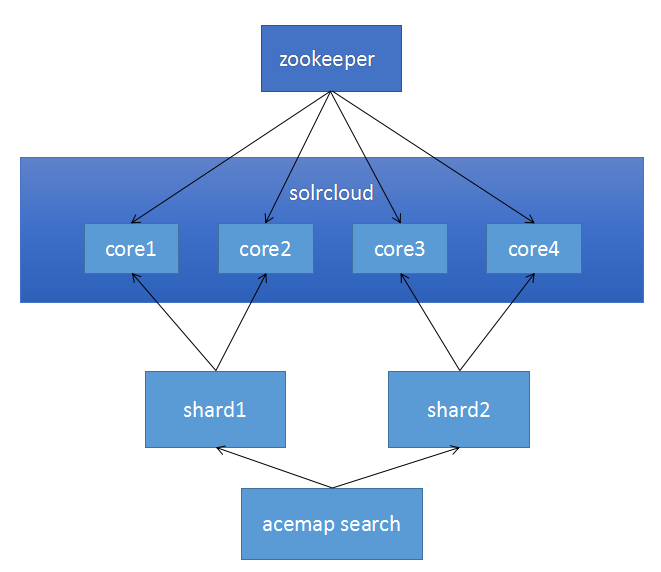
\includegraphics[width=0.6\textwidth]{zookeeper.png}
  \bicaption[fig:solrcloud]{云服务器初始架构}{云服务器初始架构}{Fig.}{Solrcloud Simplified}
\end{figure}

在这里,我们把原来单一的Solr实例(Instance,又叫Core)分为四个节点,并由一个Zookeeper服务器进行统一管理。同时,我们原本的单一索引文件被分成了两个片(Shard),每一个片分为两个相同的备份。这样一来,每个Solr节点里恰保存一份索引,并负责与该份索引相关的索引工作。我们将Core1与Core3放在同一台服务器上,Core2个Core4放在另一台服务器上,四台服务器上的两片索引文件和两片备份索引文件共同组成了索引集合(Collection)。

由于在实例中保存的配置文件难以同步修改,因此在这四个Solr实例中均不保存任何配置文件,所有的配置文件我们统一保存在Zookeeper的数据节点中。在索引构建的阶段,四个实例分别读取Zookeeper数据节点中的配置文件,确定自己的索引结构,并由Zookeeper内部算法决定将每一篇文档转发到哪个分片中进行索引;在查询阶段,Zookeeper决定将查询请求分配给哪些较为空闲的节点,并通过配置文件决定给Solr实例的查询请求格式,由选举出的主实例(Leader)进行结果整合与发布。

当四个节点中的任意一个节点因为意外(例如索引文件损坏,进程意外终止等)无法正常工作时,Zookeeper会自动检测到节点的异常,并将其标记为宕机(Down)状态或离线(Gone)状态,此时整个系统的服务并不会终止,而是会由剩下的节点分配承担所有任务。由于目前架构中任意一台服务器上都保存着一份所有索引的备份,所以只要不是所有的计算机服务器全部宕机,完整的服务功能都会保持。当意外关闭的节点被重新注册回Zookeeper时,Zookeeper会尝试恢复该节点并使其回复正常工作。

以上的架构看似很完美,然而仍然存在一个严重的缺陷——那就是Zookeeper节点的单一性会导致其反而成为系统鲁棒性的短板。换句话说,虽然对于目前的架构任意Solr节点的宕机都不会造成服务故障,但是一旦Zookeeper服务本身出现故障,所有的服务都会跟着瘫痪。解决这一问题的方法有两个,一是将Zookeeper服务运行在几乎不需要维护重启的专门服务器上,二是针对Zookeeper服务器本身建立一个分布式架构。用通俗的话说,第二种解决问题的方法,就是用Zookeeper Cloud来管理Solr Cloud。该改进的架构如下图所示:
\begin{figure}[!htp]
  \centering
  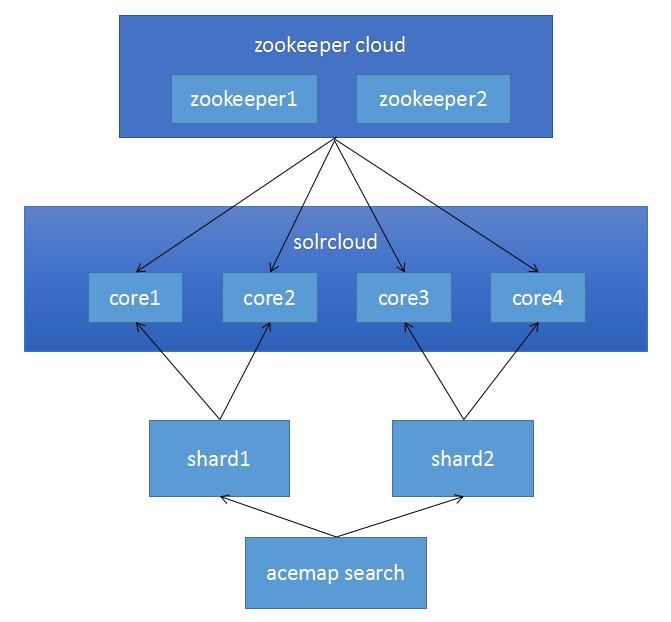
\includegraphics[width=0.6\textwidth]{zookeepercloud.png}
  \bicaption[fig:solrcloudadv]{云服务器改进架构}{云服务器改进架构}{Fig.}{Solrcloud Advanced}
\end{figure}
此时,Zookeeper不仅管理着四个Solr节点,同时也管理着两个Zookeeper节点。与Solr节点自动选取Leader类似,Zookeeper节点的Leader也是由内部自动选举得到的。两个Zookeeper节点的存在分担了Zookeeper服务器宕机的风险,使得其中任何一个Zookeeper服务器故障都不会影响到系统整体的正常工作。一个显而易见的好处是,在这个架构下我们可以只配置两台服务器计算机,并在每台计算机上部署一个Zookeeper节点和两个Solr节点,此时任何一台计算机的重启都不会终止服务的正常提供。而如果不配置两个Zookeeper节点,运行着Zookeeper服务的计算机是不能重启的,否则整个服务就会崩溃。

但是这个方案和第一套方案相比也不是十全十美的。第一套解决方案能保证系统在上线后,能够用一套十分简单的流程来维护系统的所有功能,而对于第二套解决方案架构的系统,其维护过程会比第一套解决方案复杂很多,在非专业人士操作维护时可能会让服务器产生更多的故障。因此这里只是在理论上说明了第二套流程的可行性及其优势,在实际搜索平台的实现中,我们并没有采用云架构部署Zookeeper本身。

\section{分布式系统的部署}
这一部分介绍云服务器初始架构的部署方式。具体的部署命令可以参见附录1中,上面有详细的罗列。

首先,我们需要配置并启动一个Zookeeper服务。Zookeeper服务的配置需要指定5个参数,我们通过修改zoo.cfg文件以完成此处的配置。
\begin{enumerate}
\item tickTime:一次同步的时间周期,此处设置为2000ms;
\item initLimit:第一次同步过程花费时间周期数的限制,此处设置为10;
\item syncLimit:一次同步过程的时间周期数限制,即发送请求与得到相应之间的最大周期数间隔,此处设置为5;
\item dataDir:存放快照数据的目录,根据需要设置;
\item clientPort:服务运行的端口,所有的Solr节点都要通过这个端口注册到Zookeeper。
\end{enumerate}

配置好这些参数后,我们就可以启动Zookeeper服务了。启动Zookeeper服务后,我们可以打开其客户端(Client)查看内部文件情况,由于是新挂载的节点,所以里面是没有任何文件的。针对之后需要挂载的Solr服务,需要在Zookeeper上挂载一个空节点,这里起名为acemap节点。

接下来要将Solr服务器注册到Zookeeper上。我们在两台服务器上各启动一个Solr服务,然后在每一个Solr服务上运行两个实例节点。在这一过程中,首先需要配置Solr服务的host地址,由于本平台中两台服务器并不在同一个内网上,所以我们使用公网地址作为服务的Solr地址。然后,我们需要指定服务以云模式启动并挂在到Zookeeper的acemap节点上,并指定为其Java虚拟机分配的内存。

第一台服务器上的Solr服务启动后,Zookeeper的acemap节点上会自动保存一些基本的配置文件,打开其中的live\_nodes文件夹,可以看到对应与启动服务host名称的记录文件。启动第二台服务器上的Solr服务后,live\_nodes文件夹里会显示两个服务各自的记录文件。

之后,我们需要在两个Solr服务组成的集群上创建一个新的索引集合(Collection),并以2的冗余度创建两个分片。此时,这四个分片会被自动分配到四个Solr节点中,同时每台服务器上的Solr服务都会自动分配到两个不同的分片。

最后,我们需要实现配置文件的统一管理功能。这一功能可以借助zkcli.sh进行实现。我们先将所有的配置文件统一放入文件夹中,用zkcli.sh的upconfig方法可以将本地的文件夹传入Zookeeper对应节点上,downconfig方法可以将Zookeeper节点上的文件下载到本地。在文件夹被挂载到节点上之后,我们可以用linkconfig函数将节点与Solr云中的collection对应起来。

至此,Solr服务器的分布式部署已经基本完成,我们可以通过访问任何一个Solr服务器来管理这个分布式的集合(collection)。

\section{分布式系统的配置}
分布式系统的配置方法和单台服务器的配置方法大同小异。在集合整体的视角下,四个子节点组成的整体可以视作一个大的单台服务器,因此,系统配置的过程和单台服务器一样,需要先配置solrconfig.xml文件,再进行索引结构设计与文档导入,最后进行查询指令的设计。不同的是,在配置文件与索引结构设计完成后,注意需要用reload指令确保指令被同步到了每个节点之中。

此外,由于索引被分成了两个独立的片,因此查询指令中新增了一条\&shard=XXX的命令,用以只在某个片中搜索结果。更进一步地,可以指定只在某个shard的某个特定的备份中进行查询。这种查询方式称作分布式查询。(参考资料https://cwiki.apache.org/confluence/display/solr/Distributed+Requests)

既然Solr云架构拥有分布式查询的功能,那就说明shard的构建过程除了交给系统自动进行外,也可以人为地进一步自定义。例如,在集合创建时,可以用router.name属性在决定每一条文档被分发到哪一个具体的片上。例如对于本学术网站的搜索平台,router.name可以由论文属于计算机领域或是非计算机领域决定,通过将计算机领域的论文索引到其中一个片,非计算机领域的论文索引到另一个片,就可以用分布式查询的方法高效的在计算机或非计算机论文这两个子集中分别查询论文。但是由于实际上非计算机领域和计算机领域论文这一划分方式并不均匀,前者的数量实际上会远远多于后者,所以会导致资源分配不均匀的问题。我们可以通过添加服务器,并利用片分割(Shard Splitting)的方法将较大的片进一步分割存储到更多的服务器中,以达到负载均衡。
%# -*- coding: utf-8-unix -*-
%%==================================================
%% chapter01.tex for SJTU Master Thesis
%%==================================================

%\bibliographystyle{sjtu2}%[此处用于每章都生产参考文献]
\chapter{基于查询系统的知识图设计}
\label{chap:c6}
\section{背景知识}
知识图谱是将知识整合后以图的形式表现的一种方法,也是一种可视化的知识管理工具。在毕设开题报告的时候,我就一直思考如何为我的偏工程的设计中发掘出一些理论意义,于是便有了这个结合查询系统进行知识图设计的想法。该功能的构想基于如下考量:用户使用学术网站进行查询的时候,可能只重点关注搜索结果的前几条,而隐藏在大量搜索结果之中的信息则无法很好的被用户知晓。论文希望设计出一套根据用户输入的查询关键词动态生成知识图,帮助用户发掘出这些埋藏的信息。例如对于用户可能对“节能”这一关键词感兴趣,于是他键入这一关键词并查询,系统则能在环境科学、经济学、电气、化学、数学等领域梳理出相关研究的层级状知识图,以帮助用户更好地确定与了解自己的研究方向。

\begin{figure}[!htp]
  \centering
  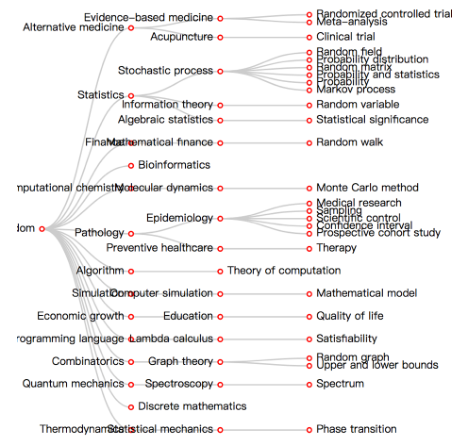
\includegraphics[width=0.6\textwidth]{knowledgegraph.png}
  \bicaption[fig:knowledgegraph]{一个简单的层级状知识图}{一个简单的层级状知识图}{Fig.}{A simple layered knowledge graph}
\end{figure}

为了更好地说明我的设计目标,我绘制了一个简单的层级状知识图作为示例。如图所示,对于用户输入的关键词random,我们可以看到几棵规模较大的子树,例如Alternative Medicine(替代医学),Statistics(统计学),Pathology(病理学)等;也有一些规模不大但是我个人比较感兴趣的子树,例如Algorithm(算法)和Programming Language(编程语言)等;同时,还有Quantum Mechanics(量子力学)等重要的学科子树。这些子树又扩展开,给我们展示了这些领域的子领域相关知识。

此图是基于用户搜索random这一关键词,根据查询结果动态生成的。显然,该图相比单纯的查询结果列表能反映出更多的信息。例如,“随机”这一关键词在医学领域的应用比在计算机领域要更加地广泛,并且和统计学密切相关。如果一个研究者对“随机”这一关键词感兴趣,他如果作为一名应用科学的从业者,那么可以更多的了解到理论科学方面统计学的相关的知识点,并作为自己的研究工具;如果他是一名理论科学的从业者,也可以通过了解到随机这一关键词在医学与计算机科学方面的应用,从而给自己理论的实际应用带来灵感。这就是根据用户搜索的内容来动态生成知识图的应用。目前的主流学术网站上很少有与该设想相重复的功能,这也是我继续这一研究的一大动力。

在理论方面,有很多的论文为我研究这一问题起到了很大的启发作用。Ronen Feldman的文章\citen{mtukd}介绍了根据实体的关键词分布进行数据挖掘的各种算法,为如何从理论的角度量化研究论文的关键词信息提供了很大的启发;Hsin-Ning Su的论文\citen{mksbk}介绍了从关键词的共现性绘制知识结构的方法,并讨论了该方法在二维知识图绘制中的应用;Yuefeng Li的论文\citen{mofaa}通过分析关键词的相关性和非相关性给出了关键词信息的筛选手段,对我们的图规模控制算法起到了启发作用;Stanley Loh的论文\citen{cbkdi}给出了关键词相关性的置信度算法,为我们对关键词之间相关性的计算给出了启发。

有了这些理论基础,我们就可以从最简单的层级状知识图入手设计我们的动态知识图生成功能。

\section{知识图生成基础算法}
与背景知识的示例中一样,我们利用查询结果中的论文关键词信息绘制层级状知识图。在这里,本文章的第4.2章中介绍的结果统计功能(facet)恰好能为我们所用。结果统计功能恰好统计了论文的关键词信息,其基本结构如下:
\begin{lstlisting}[caption={关键词结果统计}, label=kwfacet, escapeinside="", numbers=none]
{
"facet\_counts":{
    "facet\_queries":{},
    "facet\_fields":{
      "PaperPublishYear":[.....],
      "KeywordID":[
        "017C8A77",9940,
        "08EE83EF",5945,
        "09AEBB9C",4648,
        "200524E7",4165,
        .....],
      .....},
    "facet\_ranges":{},
    "facet\_intervals":{},
    "facet\_heatmaps":{}}
}
\end{lstlisting}

其中,KeywordID虽然用不直观的十六进制字符串的形式表示,但是在数据库中能很方便的查询到ID对应的实际内容,经过转化后如下:
\begin{lstlisting}[caption={关键词结果统计\_新}, label=kwfacet2, escapeinside="", numbers=none]
{
    "KeywordID":[
      "Water content",9940,
      "Chemical composition",5945,
      "Content analysis",4648,
      "Nitrogen",4165,
      .....]
}
\end{lstlisting}

在此图中我们便可以很明确地看到关键词结果统计的详细信息,我们的查询语句为“content”,而查询结果论文拥有关键词排名的前几名都与化学成分分析等领域密切相关。上表也正是一张包含了“content”这一单词的论文的关键词出现频率的排行榜。

我们的数据库中还有一张记录了关键词之间层级关系的表,它记录了每个在论文中出现过的关键词,其所在的层级(L0, L1, L2, L3)与关键词的父关键词,其中L3为最细分的层级,而L0为最概括的层级。结合这张表的内容,我们即可以实现知识图生成的基础算法。首先,我们说明如何生成一颗基础的树状知识图:

\begin{algorithm}
% \begin{algorithm}[H] % 强制定位
\caption{生成基础的树状知识图}
\label{getrawtree}
\begin{algorithmic}[1] %每行显示行号
\Ensure 树状知识图$knowledgetree$ % 输出
\Require 用户查询关键词$userinput$, 结果统计关键词列表$keylist$, 关键词层级关系表$hierarchy$ % 输入
\State $knowledgetree \gets \{\}$
\State $root \gets userinput$
\State $knowledgetree.append(root)$
\For{$node$ in $keylist$}
  \State $node.parent \gets hierarchy[node]$
  \If {$node$ not in $knowledgetree$ and $node.parent==None$}
    \State $node.parent \gets root$
    \State $knowledgetree.append(node)$
  \EndIf
  \If {$node$ not in $knowledgetree$ and $node.parent != None$}
    \State $nodep \gets node.parent$
    \State $knowledgetree.append(node)$
    \State $keylist.append\{nodep\}$
  \EndIf
\EndFor
\end{algorithmic}
\end{algorithm}

通过该算法,我们可以得到得到一棵理论上信息完全的知识图树结构,但是其保存的数据结构还略显混乱,因此我们需要进一步将之前得到的数据结构进行格式化。一个好的树的数据结构应该是这样的:

\begin{lstlisting}[caption={树数据结构}, label=treestructure, escapeinside="", numbers=none]
{node:{
  nodeproperty1 : aaa,
  nodeproperty2 : bbb,
  ...,
  children:{node*}
  }
}
\end{lstlisting}

在该数据结构中,树用一个字典进行表示,字典中只有一个键为根节点的元素,其值为根节点的各种属性与子节点列表。子节点字典要么为空,要么包含的元素递归地为与根节点相同的字典结构。

上述优结构的树与算法6-1得到的树最大的区别在于,优结构树中父节点总是在子节点之前出现的,而算法6-1得到的树的父节点会经常地在子节点之后出现。可以运用递归函数,用栈的思想即可将算法6-1得到的输出转化为上述优字典结构的树。具体实现此处略去。

得到了优结构的树后,我们即可以开始考虑知识图的绘制问题。

\section{知识图的绘制}
我们使用数据可视化工具d3.js来进行知识图的绘制。d3是数据驱动文档(Data Driven Document)的简称,它以开源Javascript代码的形式提供了很多方便的网页数据可视化接口。d3.js提供了许多绘制层级状树结构的示例接口。例如图6.1的系统树图(Dendrogram),下图所示的径向树(Radial tree)与放射图(sunburst)等。

\begin{figure}[!htp]
  \centering
  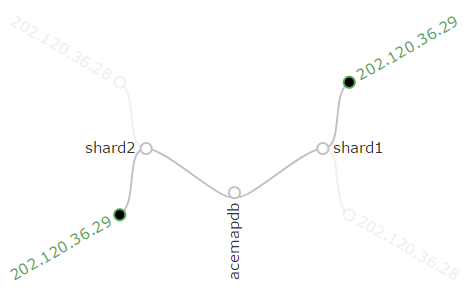
\includegraphics[width=0.3\textwidth]{radial.png}
  \hspace{1cm}
  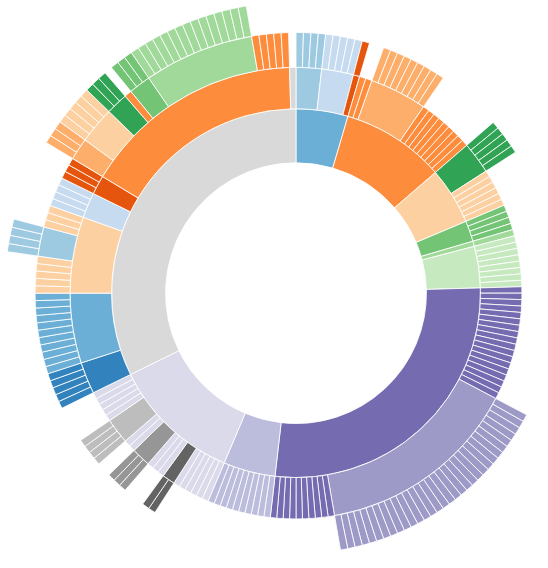
\includegraphics[width=0.3\textwidth]{sunburst.png}
  \bicaption[fig:sunburst]{径向树与放射图}{左:径向树;右:放射图}{Fig}{radial tree and sunburst}
\end{figure}

这些工具都可以用来展示层级状知识图,但是以上两幅图相比图\ref{fig:knowledgegraph}的传统树状图,对空间的利用率更高,且支持更多的用户交互动作,因此更适合在网站中使用。运用这些接口绘制我们的我们的层级状知识图,图上的圆心代表用户查询的关键词,而图上的同心圆从内到外依次代表树节点各层次的内容 。实际绘制得到的效果如图\ref{fig:sunburst2}所示。

\begin{figure}[!htp]
  \centering
  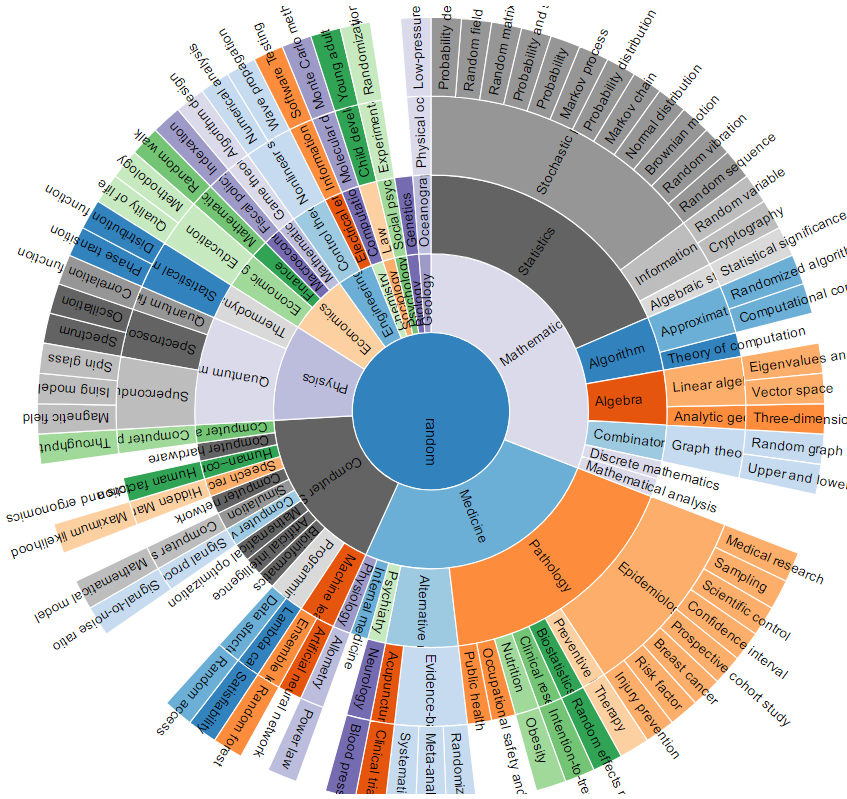
\includegraphics[width=0.45\textwidth]{sunburst2.png}
  \hspace{1cm}
  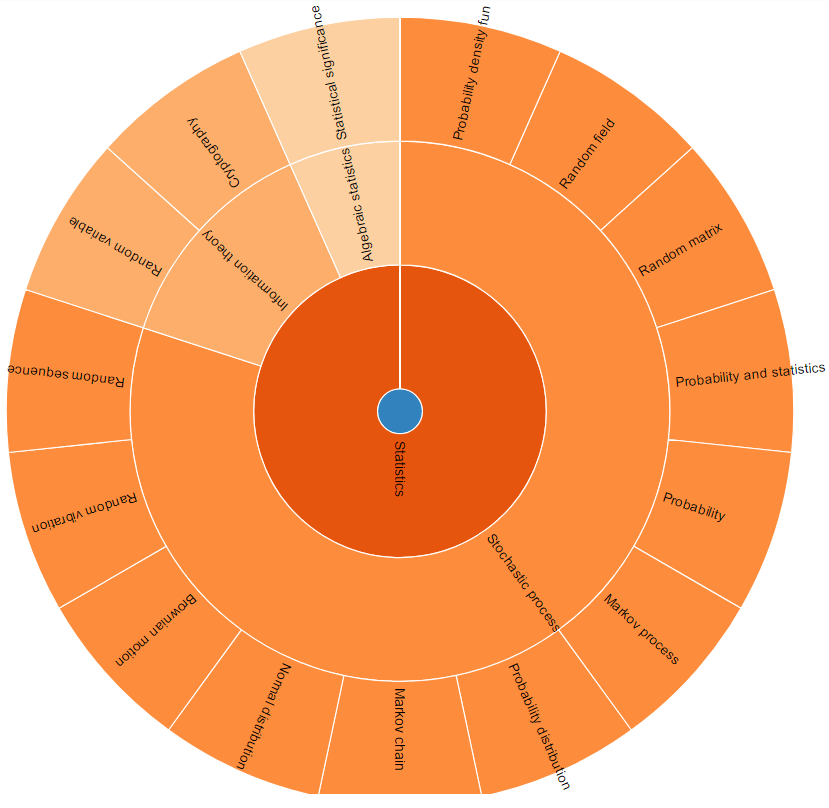
\includegraphics[width=0.45\textwidth]{sunburst3.png}
  \bicaption[fig:sunburst2]{放射状知识图与知识图子树}{左:放射状知识图;右:知识图子树}{Fig}{sunburst and subtree sunburst}
\end{figure}

图\ref{fig:sunburst2}中左图是算法6-1得到的树结构化后直接绘制的知识图,右图是将左图两点钟方向的子树放大后的效果。可以看出,绘制的知识图已经有了初步的雏形与信息量,但是也存在着明显的问题。左图包含的节点数显然过多,左半部分有大量紧密的难以阅读的节点;而右图包含的节点数又太少,使得放射图的表现效果不佳。因此,下一步我们需要进行知识图的规模控制,将知识图的节点数控制在一个合适的水平。

\section{知识图规模的控制}
我们用以下三种算法实行知识图规模的控制:
\subsection{去除信息缺失的节点}
我们生成的知识图以树的形式呈现,其中树的根节点是人为加入的参考节点。去除根节点,可以得到一组树${T_1,T_2,...T_n}$。这些树中的节点均为论文的关键词节点,节点包含层级信息${L_0,L_1,L_2,L_3}$,代表关键词节点在论文关键词层级表中处于哪一层。考虑图\ref{fig:sunburst2}中的左半部分,其中包含了一些直接连接至根节点的$L_2,L_3$层节点,它们同时也是子树集合${T_1,T_2,...T_n}$的根节点。我们认为,直接连接至根节点的$L_2,L_3$层节点处于较为细化的层次,其子节点层数至多为一层,且很有可能是因为数据库信息缺失导致的父节点信息丢失。这些信息缺失的节点会影响对整张图层级化结构的认识,因此我们将这些节点联通其连接的树结构删去。详见算法\ref{ago1}。

\begin{algorithm}
% \begin{algorithm}[H] % 强制定位
\caption{去除信息缺失的节点}
\label{ago1}
\begin{algorithmic}[1] %每行显示行号
\Ensure 子树集合$\{T_1',T_2',...T_m'\}$ % 输出
\Require 原始树集合$\{T_1,T_2,...T_n\}$ % 输入
\For{$t$ in $\{T_1,T_2,...T_n\}$}
  \State $troot \gets t.root$
  \If {$troot.layer==L2$ or $troot.layer==L3$}
    \State remove $t$ from $\{T_1,T_2,...T_n\}$
  \EndIf
\EndFor
\end{algorithmic}
\end{algorithm}

\subsection{去除信息缺失的节点}

\section{知识图的显示效果}
我们运用以上算法保留有用节点,并删除了一些重要性相对较低的节点,目的就是把最终知识图的规模控制到合理的范围内。因为是动态生成层级状知识图的算法,所以我们没有采用高复杂度的算法,而是更加重视算法在系统上的响应速度,以保证该功能可以顺利上线。经过测试,本方法在知识图的规模控制上有着很好的效果。为了进一步丰富展示的内容,我们用放射图圆弧的弧度直观显示对应关键词的对应论文数目,并将论文数量随年份的演化关系在图右侧的折线图上显示。

如图,运用d3.js提供的交互式脚本我们实现了知识图的最终效果。在知识图的规模被合理化的同时,系统会跟踪用户鼠标指针的位置,并显示鼠标指向的块的层次关系和其对应的关键词论文数随时间的变化趋势。至此,基于查询系统的知识图设计功能即完成实现。
%# -*- coding: utf-8-unix -*-
%%==================================================
%% conclusion.tex for SJTUThesis
%% Encoding: UTF-8
%%==================================================

\begin{summary}

本次毕设课题的工作成功地完成了Acemap的2.0版搜索平台的部署。2.0版本的查询系统成功解决了在1.0版本中存在的查询速度与索引速度严重不足和功能缺乏的问题。对于查询速度不足的问题,我采用了将索引文件映射到内存的方法,成功将查询的速度相对原查询系统相比提升了三倍以上;对于索引速度不足的问题,我采用了文件导入法代替数据库导入法,将索引的平均速度提高了超过一百倍,实现了完整索引的成功建立。在另一方面,我实现了查询系统的分布式部署,成功在两台服务器上搭建了系统的分布式云服务,进一步强化了搜索引擎的搜索性能与稳定性。搜索平台的部署工作到此便告一段落,基本的平台维护方式我都整理到了论文的附录中,可以参照附录进行系统的后期维护。

在知识图方面,我一开始的想法是作出一个强理论性的系统,同时也要兼顾系统的展示效果。但是在实际操作中,不同种类的图的展示效果千差万别,并没有一个固定的理论去说按什么标准组织的图的展示效果是最好的,所以后来这部分的工作中,展示效果的优化成了工作的重点,理论部分的工作反而相对随性,只是根据一些参考论文的思想构建了一套自己的规模控制算法,并在自己的系统中使用。由于最终的目标是完成知识图的动态生成,根据用户的输入查询语句直接反馈出相应的知识图,所以算法的复杂度的限制相当高,很多迭代算法因为收敛速度不够也因之被弃用。在论文使用的算法中,使用了一次递归的规模值计算算法和收敛速度较快的Kmeans算法,算法复杂度并不高,在实际应用中也有着较好的效果。

很高兴本次毕设课题的任务书中的都能够被圆满地解决,在解决一个个实际问题的过程中,我对搜索引擎这一应用有了更全面的认识,也学到了各种算法与软件方面的知识。感谢这次毕业设计的机会,让我有了许多收获,也激励我在今后研究生阶段的学习和工作中虚心学习,勇于面对一切困难与挑战。
\end{summary}


\appendix	% 使用英文字母对附录编号,重新定义附录中的公式、图图表编号样式
\renewcommand\theequation{\Alph{chapter}--\arabic{equation}}	
\renewcommand\thefigure{\Alph{chapter}--\arabic{figure}}
\renewcommand\thetable{\Alph{chapter}--\arabic{table}}
\renewcommand\thealgorithm{\Alph{chapter}--\arabic{algorithm}}

%% 附录内容,本科学位论文可以用翻译的文献替代。
%%# -*- coding: utf-8-unix -*-
\chapter{搭建模板编译环境}

\section{安装TeX发行版}

\subsection{Mac OS X}

Mac用户可以从MacTeX主页\footnote{\url{https://tug.org/mactex/}}下载MacTeX 2015。
也可以通过brew包管理器\footnote{\url{http://caskroom.io}}安装MacTeX 2015。

\begin{lstlisting}[basicstyle=\small\ttfamily, numbers=none]
brew cask install mactex
\end{lstlisting}

\subsection{Linux}

建议Linux用户使用TeXLive主页\footnote{\url{https://www.tug.org/texlive/}}的脚本来安装TeXLive 2015。
以下命令将把TeXLive发行版安装到当前用户的家目录下。
若计划安装一个供系统上所有用户使用的TeXLive,请使用root账户操作。

\begin{lstlisting}[basicstyle=\small\ttfamily, numbers=none]
wget http://mirror.ctan.org/systems/texlive/tlnet/install-tl-unx.tar.gz
tar xzvpf install-tl-unx.tar.gz
cd install-tl-20150411/
./install-tl
\end{lstlisting}

\section{安装中文字体}

\subsection{Mac OS X、Deepin}

Mac和Deepin用户双击字体文件即可安装字体。

\subsection{RedHat/CentOS用户}

RedHat/CentOS用户请先将字体文件复制到字体目录下,调用fc-cache刷新缓存后即可在TeXLive中使用新字体。

\begin{lstlisting}[basicstyle=\small\ttfamily, numbers=none]
mkdir ~/.fonts
cp *.ttf ~/.fonts				# 当前用户可用新字体
cp *.ttf /usr/share/fonts/local/	# 所有用户可以使用新字体
fc-cache -f
\end{lstlisting}


%%# -*- coding: utf-8-unix -*-
%% app2.tex for SJTU Master Thesis
%% based on CASthesis
%% modified by wei.jianwen@gmail.com
%% version: 0.3a
%% Encoding: UTF-8
%% last update: Dec 5th, 2010
%%==================================================

\chapter{Maxwell Equations}

选择二维情况,有如下的偏振矢量:
\begin{subequations}
  \begin{eqnarray}
    {\bf E}&=&E_z(r,\theta)\hat{\bf z} \\
    {\bf H}&=&H_r(r,\theta))\hat{ \bf r}+H_\theta(r,\theta)\hat{\bm
      \theta}
  \end{eqnarray}
\end{subequations}
对上式求旋度:
\begin{subequations}
  \begin{eqnarray}
    \nabla\times{\bf E}&=&\frac{1}{r}\frac{\partial E_z}{\partial\theta}{\hat{\bf r}}-\frac{\partial E_z}{\partial r}{\hat{\bm\theta}}\\
    \nabla\times{\bf H}&=&\left[\frac{1}{r}\frac{\partial}{\partial
        r}(rH_\theta)-\frac{1}{r}\frac{\partial
        H_r}{\partial\theta}\right]{\hat{\bf z}}
  \end{eqnarray}
\end{subequations}
因为在柱坐标系下,$\overline{\overline\mu}$是对角的,所以Maxwell方程组中电场$\bf E$的旋度:
\begin{subequations}
  \begin{eqnarray}
    &&\nabla\times{\bf E}=\mathbf{i}\omega{\bf B} \\
    &&\frac{1}{r}\frac{\partial E_z}{\partial\theta}{\hat{\bf
        r}}-\frac{\partial E_z}{\partial
      r}{\hat{\bm\theta}}=\mathbf{i}\omega\mu_rH_r{\hat{\bf r}}+\mathbf{i}\omega\mu_\theta
    H_\theta{\hat{\bm\theta}}
  \end{eqnarray}
\end{subequations}
所以$\bf H$的各个分量可以写为:
\begin{subequations}
  \begin{eqnarray}
    H_r=\frac{1}{\mathbf{i}\omega\mu_r}\frac{1}{r}\frac{\partial
      E_z}{\partial\theta } \\
    H_\theta=-\frac{1}{\mathbf{i}\omega\mu_\theta}\frac{\partial E_z}{\partial r}
  \end{eqnarray}
\end{subequations}
同样地,在柱坐标系下,$\overline{\overline\epsilon}$是对角的,所以Maxwell方程组中磁场$\bf H$的旋度:
\begin{subequations}
  \begin{eqnarray}
    &&\nabla\times{\bf H}=-\mathbf{i}\omega{\bf D}\\
    &&\left[\frac{1}{r}\frac{\partial}{\partial
        r}(rH_\theta)-\frac{1}{r}\frac{\partial
        H_r}{\partial\theta}\right]{\hat{\bf
        z}}=-\mathbf{i}\omega{\overline{\overline\epsilon}}{\bf
      E}=-\mathbf{i}\omega\epsilon_zE_z{\hat{\bf z}} \\
    &&\frac{1}{r}\frac{\partial}{\partial
      r}(rH_\theta)-\frac{1}{r}\frac{\partial
      H_r}{\partial\theta}=-\mathbf{i}\omega\epsilon_zE_z
  \end{eqnarray}
\end{subequations}
由此我们可以得到关于$E_z$的波函数方程:
\begin{eqnarray}
  \frac{1}{\mu_\theta\epsilon_z}\frac{1}{r}\frac{\partial}{\partial r}
  \left(r\frac{\partial E_z}{\partial r}\right)+
  \frac{1}{\mu_r\epsilon_z}\frac{1}{r^2}\frac{\partial^2E_z}{\partial\theta^2}
  +\omega^2 E_z=0
\end{eqnarray}

%%# -*- coding: utf-8-unix -*-
\chapter{从 \CJKLaTeX 转向 \XeTeX }
\label{chap:whydvipdfm}

我习惯把v0.2a使用dvipdfmx编译的硕士学位论文模板称为“ \CJKLaTeX 模板”,而这个使用 \XeTeX 引擎(xelatex程序)处理的模板则被称为“{\XeTeX/\LaTeX}模板”。
从 \CJKLaTeX 模板迁移到{\XeTeX\LaTeX}模板的好处有下:
\begin{enumerate}
\item[\large\smiley] 搭建 \XeTeX 环境比搭建 \CJKLaTeX 环境更容易;
\item[\large\smiley] 更简单的字体控制;
\item[\large\smiley] 完美支持PDF/EPS/PNG/JPG图片,不需要“bound box(.bb)”文件;
\item[\large\smiley] 支持OpenType字体的复杂字型变化功能;
\end{enumerate}

当然,这也是有代价的。由于 \XeTeX 比较新,在我看来,使用 \XeTeX 模板所必须付出的代价是:

\begin{enumerate}
\item[\large\frownie] 必须把你“古老的” \TeX 系统更新为较新的版本。TeXLive 2012和CTeX 2.9.2能够编译这份模板,而更早的版本则无能为力。
\item[\large\frownie] 需要花一些时间把你在老模板上的工作迁移到新模板上。
\end{enumerate}

第一条就看你如何取舍了,新系统通常意味着更好的兼容性,值得升级。而转换模板也不是什么特别困难的事情,可以这样完成:

\begin{enumerate}
\item 备份你要转换的源文件,以防你的工作成果丢失;
\item 将你原来的tex以及bib文件另存为UTF-8编码的文件。iconv、vim、emacs、UEdit等等工具都可以完成。WinEdt对文件编码识别功能很差(到了v6.0还是如此),不推荐作为字符编码转换工具;
\item 将diss.tex导言区中的内容替换为XeTeX模板diss.tex导言区的内容;
\item 将你对原先导言区的修改,小心翼翼地合并到新的导言区中;
\item 使用XeTeX模板中的GBT7714-2005NLang.bst替换原有的bst文件,新的bst文件只是将字符编码转换为UTF-8;
\item 删除bouding box文件;
\item 使用本文\ref{sec:process}介绍的方法,重新编译文档;
\end{enumerate}


%%# -*- coding: utf-8-unix -*-
\chapter{模板更新记录}
\label{chap:updatelog}

\textbf{2016年12月} v0.9.5发布,改用GB7714-2015参考文献风格。

\textbf{2016年11月} v0.9.4发布,增加算法和流程图。

\textbf{2015年6月19日} v0.9发布,适配ctex 2.x宏包,需要使用TeXLive 2015编译。

\textbf{2015年3月15日} v0.8发布,使用biber/biblatex组合替代 \BibTeX ,带来更强大稳定的参考文献处理能力;添加enumitem宏包增强列表环境控制能力;完善宏包文字描述。

\textbf{2015年2月15日} v0.7发布,增加盲审选项,调用外部工具插入扫描件。

\textbf{2015年2月14日} v0.6.5发布,修正一些小问题,缩减git仓库体积,仓库由sjtu-thesis-template-latex更名为SJTUThesis。

\textbf{2014年12月17日} v0.6发布,学士、硕士、博士学位论文模板合并在了一起。

\textbf{2013年5月26日} v0.5.3发布,更正subsubsection格式错误,这个错误导致如"1.1 小结"这样的标题没有被正确加粗。

\textbf{2012年12月27日} v0.5.2发布,更正拼写错误。在diss.tex加入ack.tex。

\textbf{2012年12月21日} v0.5.1发布,在 \LaTeX 命令和中文字符之间留了空格,在Makefile中增加release功能。

\textbf{2012年12月5日} v0.5发布,修改说明文件的措辞,更正Makefile文件,使用metalog宏包替换xltxtra宏包,使用mathtools宏包替换amsmath宏包,移除了所有CJKtilde(\verb+~+)符号。

\textbf{2012年5月30日} v0.4发布,包含交大学士、硕士、博士学位论文模板。模板在\href{https://github.com/weijianwen/sjtu-thesis-template-latex}{github}上管理和更新。

\textbf{2010年12月5日} v0.3a发布,移植到 \XeTeX/\LaTeX 上。

\textbf{2009年12月25日} v0.2a发布,模板由CASthesis改名为sjtumaster。在diss.tex中可以方便地改变正文字号、切换但双面打印。增加了不编号的一章“全文总结”。
添加了可伸缩符号(等号、箭头)的例子,增加了长标题换行的例子。

\textbf{2009年11月20日} v0.1c发布,增加了Linux下使用ctex宏包的注意事项、.bib条目的规范要求,
修正了ctexbook与listings共同使用时的断页错误。

\textbf{2009年11月13日} v0.1b发布,完善了模板使用说明,增加了定理环境、并列子图、三线表格的例子。

\textbf{2009年11月12日} 上海交通大学硕士学位论文 \LaTeX 模板发布,版本0.1a。


%# -*- coding: utf-8-unix -*-
\chapter{搜索平台的启动和维护命令}

\section{单机版架构}
\subsection{启动服务}
单机版服务的启动可以直接使用example中的data import handler示例,启动方式为:
\begin{lstlisting}[basicstyle=\small\ttfamily, numbers=none]
cd solr-6.5.0
bin/solr -e dih -m 20g
\end{lstlisting}

其中-e dih指启动data import handler这一example,-m为JAVA虚拟机分配内存。启动后,基本功能都已经配置完成,接下来可以从索引结构设计开始进行进一步配置。

当然,用示例启动服务器这一行为并不优雅,我们可以用下面的指令启动一个正式的服务器:
\begin{lstlisting}[basicstyle=\small\ttfamily, numbers=none]
cd solr-6.5.0
bin/solr start -h host -p port -d dir -m memory
\end{lstlisting}

用这个指令,我们可以指定host地址,端口地址和服务器文件地址,并开启一个新的未经过配置的服务。这时我们需要从头配置所有的内容,参见第二章中平台配置小节。

\subsection{关闭服务}
关闭某个端口的服务,可以用指令:
\begin{lstlisting}[basicstyle=\small\ttfamily, numbers=none]
cd solr-6.5.0
bin/solr stop -p port
\end{lstlisting}

关闭本地所有端口的服务,可以用指令:
\begin{lstlisting}[basicstyle=\small\ttfamily, numbers=none]
cd solr-6.5.0
bin/solr stop -all
\end{lstlisting}

\section{分布式架构}
\subsection{启动服务}
分布式架构中首先需要启动Zookeeper服务:
\begin{lstlisting}[basicstyle=\small\ttfamily, numbers=none]
cd zookeeper-3.4.10
bin/zkServer.sh start
\end{lstlisting}

注意服务被启动到了哪个端口,这个端口号在conf/zoo.cfg中指定,之后需要再次用到,此处假设为1234端口。启动zkCli.sh并创建一个名为acemap的新节点:
\begin{lstlisting}[basicstyle=\small\ttfamily, numbers=none]
cd zookeeper-3.4.10
bin/zkCli.sh create nodename
\end{lstlisting}

分别在两台服务器上以云模式启动Solr服务:
\begin{lstlisting}[basicstyle=\small\ttfamily, numbers=none]
On Solr Server1:
cd solr-6.5.0
bin/solr start -h s1host -cloud -p s1port -z zkhost:1234/nodename -m 20g
On Solr Server2:
cd solr-6.5.0
bin/solr start -h s2host -cloud -p s2port -z zkhost:1234/nodename -m 20g
\end{lstlisting}

其中s1host与s2host是两台服务器的主机地址,s1port和s2port是两台服务器希望启动服务的端口号,zkhost是zookeeper服务的主机地址,1234为之前指定的端口号,nodename为之前指定的节点名称。

当服务因故退出或计算机重启后,使用以上指令可以使服务重新注册回云端。

管理云平台索引集合:
\begin{lstlisting}[basicstyle=\small\ttfamily, numbers=none]
cd solr-6.5.0
增加collection:bin/solr create -c collectionname -shards 2 -replicationFactor 2
删除collection:bin/solr delete -c collectionname
\end{lstlisting}

其中-shards表示索引分片数目,-replicationFactor表示分片备份数目,一般来说,这两个值都与分布式服务器的数目相同。

更新配置文件:
\begin{lstlisting}[basicstyle=\small\ttfamily, numbers=none]
在任何一台运行了Solr服务的计算机上:
cd solr-6.5.0/server/scripts/cloud-scripts
./zkcli.sh -z zkhost:1234/nodename -cmd upconfig -confdir configdirectory -confname configname
\end{lstlisting}

其中configdirectory为存放配置文件的本地目录,configname为节点名字(一般与collection名字相同),此命令会将配置文件传到Zookeeper的名为nodename的节点上。

更新配置文件后,需要重新加载集合:
\begin{lstlisting}[basicstyle=\small\ttfamily, numbers=none]
在任何一台运行了Solr服务的计算机上:
http://solrhost:port/solr/admin/collections?action=RELOAD&name=collectionname
\end{lstlisting}

关闭Solr服务:
\begin{lstlisting}[basicstyle=\small\ttfamily, numbers=none]
cd solr-6.5.0
bin/solr stop -p port
\end{lstlisting}

关闭Zookeeper服务:
\begin{lstlisting}[basicstyle=\small\ttfamily, numbers=none]
cd zookeeper-3.4.10
bin/zkServer.sh stop
\end{lstlisting}
%# -*- coding: utf-8-unix -*-
\chapter{索引文件映射到内存的方法}

\section{定位索引文件位置}
首先我们需要知道索引文件存放的位置。一般来说,Solr的索引文件存放于文件目录的./data/index目录下
\begin{lstlisting}[basicstyle=\small\ttfamily, numbers=none]
Index: /home/path/to/solr/collection/data/index
\end{lstlisting}

\section{备份索引文件夹}
\begin{lstlisting}[basicstyle=\small\ttfamily, numbers=none]
cp ./index ./index2
\end{lstlisting}

\section{将索引文件夹挂载到内存上}
\begin{lstlisting}[basicstyle=\small\ttfamily, numbers=none]
mount -t tmpfs -o size=90g tmpfs ./index
\end{lstlisting}
该操作会花费90G内存空间,如果计算机内存空间不足,可酌情减少。不过,该值太小会导致solr服务无法启动。

\section{将索引文件拷贝回目标目录}
\begin{lstlisting}[basicstyle=\small\ttfamily, numbers=none]
cp -Rf ./index2/* ./index
\end{lstlisting}
注意不要用mv指令直接剪切并粘贴文件。因为内存中保存的文件不稳定,所以请保留一份硬盘备份。

\section{按正常方式启动Solr服务}
\begin{lstlisting}[basicstyle=\small\ttfamily, numbers=none]
./bin/solr start
\end{lstlisting}

\backmatter	% 文后无编号部分 

%% 参考资料
\printbibliography[heading=bibintoc]

%% 致谢、发表论文、申请专利、参与项目、简历
%% 用于盲审的论文需隐去致谢、发表论文、申请专利、参与的项目
\makeatletter

%%
% "研究生学位论文送盲审印刷格式的统一要求"
% http://www.gs.sjtu.edu.cn/inform/3/2015/20151120_123928_738.htm

% 盲审删去删去致谢页
\ifsjtu@review\relax\else
  %# -*- coding: utf-8-unix -*-
\begin{thanks}

  在毕业设计结束之际,我想感谢很多在毕业设计中给过我大力帮助的人。

  首先感谢甘晓莺副教授和王新兵教授对我的毕设课题的大力支持。二位老师都是网络方向的教授,我在大三的时候,就深受王新兵教授的关照,参与写作了两篇网络方向的发表于国际A类学术会议论文。得知我更大的兴趣在工程方面,且研究生阶段的研究方向是编程语言与软件工程后,二位导师大力支持我选择了与自己兴趣紧密相关的毕设课题,并在毕设过程中给了我很大的指导和帮助。

  同时,感谢傅洛伊博士对我毕业设计的监督和指导。傅博士在我知识图构思的形成过程中起到了很大的帮助与指导作用,并在每周周进展审核中给了我很多宝贵的建议。在我大四为了申请美国学校助教而忙于准备托福考试时,也给了我莫大的支持和理解。

  最后,感谢学校里的贾雨葶同学在文件导入法中提供的帮助和林特同学在知识图理论部分提供的思路,还有许多实验室同学在我不懂的各方面积极地给我答疑解惑。我们实验室的互帮互助,互相分享的氛围使我毕业设计的进行顺利了很多,也让我学到了很多知识。

\end{thanks}
 	  %% 致谢
\fi

\ifsjtu@bachelor
  % 学士学位论文要求在最后有一个英文大摘要,单独编页码
  \pagestyle{biglast}
  %# -*- coding: utf-8-unix -*-
\begin{bigabstract}
This paper discussed the problem of the implementation and optimization of large-scaled academic searching platform. To be more concise, is to implement the 2.0 version of the searching platform for the academic website Acemap. On the first prototype of the searching platform, which is implemented before this study, its indexed was incomplete and the relevant functions were insufficient. The reason for these deficiencies is the database structure had been complicated, which created a huge I/O bound for the data import process. Moreover, the over-use of example code had made it difficult to develop self defined functions.

The initial motivation of this study is to settle these problems and implement a new version of well-functioned academic searching platform. On the one hand, my paper needs to find a algorithm to accelerate the data import speed by at least 100 times. On the other hand, I want to develop a complete searching platform from zero to fit in our functional demands, and to implement it on distributed architecture to enlarge its robustness and maintainability.

On the theoretical part, this study aims to develop a knowledge graph module based on the searching platform. The target is, when users input the keyword to submit their queries, our platform can automatically generate a knowledge graph indicating the relevant academic keyword hierarchy, to better assist users for their research purpose.

Alike the 1.0 version of our search platform, we use open source search platform \emph{Solr} to develop our system. And in the distributed platform, we use \emph{Zookeeper}, a distributed service coordination platform, to manage and deposit our server nodes. Based on these tools, we implemented the 2.0 version of our search platform. This work includes the design of system architecture and index structure; fast data import algorithms. platform background and foreground development and the platform's distributed deployment. Now I will describe these works one by one.

The first work is the design of system architecture. Our system architecture contains eight parts, including the website view, website controller, query preprocess, query tokenizer, database, document preprocesser, document tokenizer and search engine server. Compared to the old version, our new version of system is having more indexed fields, which means the index structure is more complicated but supporting more query methods and richer result fields. Also, the new version implemented a complete preprocess and tokenize to the documents and queries, which handled the problem of stopwords, singular-plural pair and language tense. To speed up the query process, I used the memory project file technology to implement the file system of solr's index file folder. It is to put all the index file into memory rather than hard disk, thus making the speed of reading the index file much more faster. As a result, this new method achieved a over 3 times boost in the query speed.

The second work is fast data import algorithm. We innovatively used a file import method in the data import process thus prevented the time-consuming I/O operations. In this part we firstly exported the whole database tables to files, then we used a two level dictionary to load these files into memory. For all the data import process involving table JOIN operation, we replaced them with similar dictionary lookup operation, and we merge our all dictionaries together to form a expanded dictionary. Finally, we write our expanded dictionary into a formatted single .xml file including all the needed fields, and used this .xml file to do our data import. By changing the hard drive reading to memory reading, the data import speed is increased by over 100 times, and the difficult problem of slow data import is solved.

The third work is the platform background and foreground development. The foreground of platform is the UI interface presented as a website, and the background is the controller of the website, together with the searching platform itself. When the users' input is valid, their input on the foreground user interface is sent to the background controller, and in the background controller the query is preprocessed and sent to the search engine. Then, a HTTP response in .json format is returned back to the website controller, processed and showed in the foreground UI. Also, this part of work includes the principle of keyword highlighting and result faceting, and how these functions are implemented into the system.

The last work is the platform's distributed deployment. A singled system just works fine, but is also having its deficiencies. When the computer resource, including memory, CPU and hard disk, is highly occupied, the servers response speed will be greatly delayed. Moreover, once the server is shut down, all the service will be suddenly down and unable to work. A distributed system can solve all these problems, and a well-developed distributed system can achieve config file centralized management, workload arrangement and can handle server nodes down and recover. We used Zookeeper to implement our distributed system. In this part, we described the architecture, deployment, configure and usage of our distributed system. Our final distributed system contains 1 collection, 2 shards and 2 replicas for each shard. Each of the two server include one copy of replica for both of two shards. So, when any server shuts down, we also have one server with a complete copy of index file that can handle all the searching work. For the most time when all the 4 server nodes are alive, Zookeeper where automatically elect a leader node and the leader node will undertake the shard management and workload distribution. When any server node is dead but started again, it will also automatically login back to the cloud without any extra configuration.

After these work, the 2.0 version of searching platform is completed and can be slated to launch on the website. Then I focused on the development of the knowledge graph module. Knowledge graph is a knowledge management tool that makes organizational processes more visible, feasible, and practicable.\citen{ddm} My motivation of developing this module is stated below: When users are using an academic website, they may only focus on the top few columns of his search result. However, most information buried under thousands of more results are just ignored. So I want to develop a function to summarize and to convert these results into a visible form, and we selected the form to be a layered knowledge hierarchy graph. Detailed examples are listed in the paper. To settle this problem, we used a tree generate algorithm and tree formalization algorithm to generate the basic knowledge graph, and used a set of scale control algorithms to make sure our graph is having proper size. As we want a dynamic knowledge graph generating process, which requires a relatively low algorithm complixity and quick response, so some of the algorithms with low converge speed are not applied in the system. On the visualization of our knowledge graph, we used the sunburst effect provided by d3.js to draw it on the website. Some other elements are also added next to the graph to provide more information.

In my graduate design I successfully implemented the 2.0 version of our search system, which achieved a over 3 times query speed and a over 100 times data-import speed compared to the 1.0 version. Moreover, I implemented the whole system in distributed mode thus achieving a higher robustness and efficiency. It is glad to see all problems I want to solve having been solved well, and in the process of solving these problems, I had a more well-rounded recognition to the application of search engine. So Thanks for the chance my school providing me to have this graduate design, which have made me learned quite a lot and motivated me to be brave to face to any challenge in front of me.

\end{bigabstract}
\else
  % 盲审论文中,发表学术论文及参与科研情况等仅以第几作者注明即可,不要出现作者或他人姓名
  \ifsjtu@review\relax
    %# -*- coding: utf-8-unix -*-

\begin{publications}{3}
\end{publications}

    %# -*- coding: utf-8-unix -*-

\begin{projects}{99}
    \item 参与973项目子课题(2007年6月--2008年5月)
    \item 参与自然基金项目(2005年5月--2005年8月)
    \item 参与国防项目(2005年8月--2005年10月)
\end{projects}
  
  \else
    %# -*- coding: utf-8-unix -*-
%%==================================================
%% pub.tex for SJTUThesis
%% Encoding: UTF-8
%%==================================================

\begin{publications}{99}
\end{publications}
	      %% 发表论文
    %# -*- coding: utf-8-unix -*-
%%==================================================
%% projects.tex for SJTUThesis
%% Encoding: UTF-8
%%==================================================

\begin{projects}{99}
\end{projects}
  %% 参与的项目
  \fi
\fi

% %# -*- coding: utf-8-unix -*-
\begin{patents}{99}
    \item 第一发明人,“滑翔机”,专利申请号202510149890.0
\end{patents}
	  %% 申请专利
% \include{tex/resume}	  %% 个人简历

\makeatother

\end{document}
